\ifdefined\included
\else
\documentclass[a4paper,11pt,twoside]{StyleThese}
\usepackage{amsmath,amssymb, amsthm}             % AMS Math
\usepackage[T1]{fontenc}
\usepackage[utf8x]{inputenc}
\usepackage{babel}
\usepackage{datetime}

\usepackage{silence}

\WarningFilter{minitoc(hints)}{W0023}
\WarningFilter{minitoc(hints)}{W0028}
\WarningFilter{minitoc(hints)}{W0030}

\usepackage{lmodern}
\usepackage{tabularx}
%\usepackage{tabular}
\usepackage{multirow}
\usepackage{xspace}

\usepackage{hhline}
\usepackage[left=1.5in,right=1.3in,top=1.1in,bottom=1.1in,includefoot,includehead,headheight=13.6pt]{geometry}
\renewcommand{\baselinestretch}{1.05}

% Table of contents for each chapter

\usepackage[nottoc, notlof, notlot]{tocbibind}
\usepackage{minitoc}
\setcounter{minitocdepth}{2}
\mtcindent=15pt
% Use \minitoc where to put a table of contents

\usepackage{aecompl}

% Glossary / list of abbreviations

\usepackage[intoc]{nomencl}
\iftoggle{ThesisInEnglish}{%
\renewcommand{\nomname}{Glossary}
}{ %
\renewcommand{\nomname}{Liste des Abréviations}
}

\usepackage{etoolbox}
\renewcommand\nomgroup[1]{%
  \item[\bfseries
  \ifstrequal{#1}{A}{Number Sets}{%
  \ifstrequal{#1}{G}{Agents Beliefs and Action Models}{%
  \ifstrequal{#1}{N}{Navigation}{%
  \ifstrequal{#1}{O}{Ontology}{%
  \ifstrequal{#1}{R}{Referring Expression Generation}{%
  \ifstrequal{#1}{Z}{Controllable and Uncontrollable Agents Task Planning}{}}}}}}%
]}

\makenomenclature



% My pdf code

\usepackage{ifpdf}

\ifpdf
  \usepackage[pdftex]{graphicx}
  \DeclareGraphicsExtensions{.jpg}
  \usepackage[pagebackref,hyperindex=true]{hyperref}
  \usepackage{tikz}
  \usetikzlibrary{arrows,shapes,calc}
\else
  \usepackage{graphicx}
  \DeclareGraphicsExtensions{.ps,.eps}
  \usepackage[dvipdfm,pagebackref,hyperindex=true]{hyperref}
\fi

\graphicspath{{.}{images/}}

%% nicer backref links. NOTE: The flag ThesisInEnglish is used to define the
% language in the back references. Read more about it in These.tex

\iftoggle{ThesisInEnglish}{%
\renewcommand*{\backref}[1]{}
\renewcommand*{\backrefalt}[4]{%
\ifcase #1 %
(Not cited.)%
\or
(Cited in page~#2.)%
\else
(Cited in pages~#2.)%
\fi}
\renewcommand*{\backrefsep}{, }
\renewcommand*{\backreftwosep}{ and~}
\renewcommand*{\backreflastsep}{ and~}
}{%
\renewcommand*{\backref}[1]{}
\renewcommand*{\backrefalt}[4]{%
\ifcase #1 %
(Non cité.)%
\or
(Cité en page~#2.)%
\else
(Cité en pages~#2.)%
\fi}
\renewcommand*{\backrefsep}{, }
\renewcommand*{\backreftwosep}{ et~}
\renewcommand*{\backreflastsep}{ et~}
}

% Links in pdf
\usepackage{color}
\definecolor{linkcol}{rgb}{0,0,0.4} 
\definecolor{citecol}{rgb}{0.5,0,0} 
\definecolor{linkcol}{rgb}{0,0,0} 
\definecolor{citecol}{rgb}{0,0,0}
% Change this to change the informations included in the pdf file

\hypersetup
{
bookmarksopen=true,
pdftitle="Planning For Both Robot and Human: Anticipating and Accompanying Human Decisions",
pdfauthor="Guilhem BUISAN", %auteur du document
pdfsubject="Thèse", %sujet du document
%pdftoolbar=false, %barre d'outils non visible
pdfmenubar=true, %barre de menu visible
pdfhighlight=/O, %effet d'un clic sur un lien hypertexte
colorlinks=true, %couleurs sur les liens hypertextes
pdfpagemode=None, %aucun mode de page
pdfpagelayout=SinglePage, %ouverture en simple page
pdffitwindow=true, %pages ouvertes entierement dans toute la fenetre
linkcolor=linkcol, %couleur des liens hypertextes internes
citecolor=citecol, %couleur des liens pour les citations
urlcolor=linkcol %couleur des liens pour les url
}

% definitions.
% -------------------

\setcounter{secnumdepth}{3}
\setcounter{tocdepth}{2}

% Some useful commands and shortcut for maths:  partial derivative and stuff

\newcommand{\pd}[2]{\frac{\partial #1}{\partial #2}}
\def\abs{\operatorname{abs}}
\def\argmax{\operatornamewithlimits{arg\,max}}
\def\argmin{\operatornamewithlimits{arg\,min}}
\def\diag{\operatorname{Diag}}
\newcommand{\eqRef}[1]{(\ref{#1})}

\usepackage{rotating}                    % Sideways of figures & tables
%\usepackage{bibunits}
%\usepackage[sectionbib]{chapterbib}          % Cross-reference package (Natural BiB)
%\usepackage{natbib}                  % Put References at the end of each chapter
                                         % Do not put 'sectionbib' option here.
                                         % Sectionbib option in 'natbib' will do.
\usepackage{fancyhdr}                    % Fancy Header and Footer

% \usepackage{txfonts}                     % Public Times New Roman text & math font
  
%%% Fancy Header %%%%%%%%%%%%%%%%%%%%%%%%%%%%%%%%%%%%%%%%%%%%%%%%%%%%%%%%%%%%%%%%%%
% Fancy Header Style Options

\pagestyle{fancy}                       % Sets fancy header and footer
\fancyfoot{}                            % Delete current footer settings

%\renewcommand{\chaptermark}[1]{         % Lower Case Chapter marker style
%  \markboth{\chaptername\ \thechapter.\ #1}}{}} %

%\renewcommand{\sectionmark}[1]{         % Lower case Section marker style
%  \markright{\thesection.\ #1}}         %

\fancyhead[LE,RO]{\bfseries\thepage}    % Page number (boldface) in left on even
% pages and right on odd pages
\fancyhead[RE]{\bfseries\nouppercase{\leftmark}}      % Chapter in the right on even pages
\fancyhead[LO]{\bfseries\nouppercase{\rightmark}}     % Section in the left on odd pages

\let\headruleORIG\headrule
\renewcommand{\headrule}{\color{black} \headruleORIG}
\renewcommand{\headrulewidth}{1.0pt}
\usepackage{colortbl}
\arrayrulecolor{black}

\fancypagestyle{plain}{
  \fancyhead{}
  \fancyfoot{}
  \renewcommand{\headrulewidth}{0pt}
}

%\usepackage{MyAlgorithm}
%\usepackage[noend]{MyAlgorithmic}
\usepackage{algorithm}
\usepackage[noend]{algpseudocode}
\usepackage{comment}
\usepackage[ED=EDSYS-Robo, Ets=INSA]{tlsflyleaf}
%%% Clear Header %%%%%%%%%%%%%%%%%%%%%%%%%%%%%%%%%%%%%%%%%%%%%%%%%%%%%%%%%%%%%%%%%%
% Clear Header Style on the Last Empty Odd pages
\makeatletter

\def\cleardoublepage{\clearpage\if@twoside \ifodd\c@page\else%
  \hbox{}%
  \thispagestyle{empty}%              % Empty header styles
  \newpage%
  \if@twocolumn\hbox{}\newpage\fi\fi\fi}

\makeatother
 
%%%%%%%%%%%%%%%%%%%%%%%%%%%%%%%%%%%%%%%%%%%%%%%%%%%%%%%%%%%%%%%%%%%%%%%%%%%%%%% 
% Prints your review date and 'Draft Version' (From Josullvn, CS, CMU)
\newcommand{\reviewtimetoday}[2]{\special{!userdict begin
    /bop-hook{gsave 20 710 translate 45 rotate 0.8 setgray
      /Times-Roman findfont 12 scalefont setfont 0 0   moveto (#1) show
      0 -12 moveto (#2) show grestore}def end}}
% You can turn on or off this option.
% \reviewtimetoday{\today}{Draft Version}
%%%%%%%%%%%%%%%%%%%%%%%%%%%%%%%%%%%%%%%%%%%%%%%%%%%%%%%%%%%%%%%%%%%%%%%%%%%%%%% 

\newenvironment{maxime}[1]
{
\vspace*{0cm}
\hfill
\begin{minipage}{0.5\textwidth}%
%\rule[0.5ex]{\textwidth}{0.1mm}\\%
\hrulefill $\:$ {\bf #1}\\
%\vspace*{-0.25cm}
\it 
}%
{%

\hrulefill
\vspace*{0.5cm}%
\end{minipage}
}

\let\minitocORIG\minitoc
\renewcommand{\minitoc}{\minitocORIG \vspace{1.5em}}

\usepackage{multirow}
%\usepackage{slashbox}

\newenvironment{bulletList}%
{ \begin{list}%
	{$\bullet$}%
	{\setlength{\labelwidth}{25pt}%
	 \setlength{\leftmargin}{30pt}%
	 \setlength{\itemsep}{\parsep}}}%
{ \end{list} }

\theoremstyle{definition}
\newtheorem{definition}{Definition}
\renewcommand{\epsilon}{\varepsilon}

% centered page environment

\newenvironment{vcenterpage}
{\newpage\vspace*{\fill}\thispagestyle{empty}\renewcommand{\headrulewidth}{0pt}}
{\vspace*{\fill}}

\usepackage{tablefootnote}

\theoremstyle{plain}
\newtheorem{constraint}{Constraint}[section]

\algnewcommand\algorithmicforeach{\textbf{for each}}
\algnewcommand\algorithmicin{\textbf{in}}
\algdef{S}[FOR]{ForEach}[2]{\algorithmicforeach\ #1\ \algorithmicin\ #2\ \algorithmicdo}

\usepackage{listings}
\lstdefinestyle{customPlan}{
  language=C,
  commentstyle=\itshape\color{green!25!black},
}
\usepackage{pdfpages}

\sloppy
\begin{document}
\setcounter{chapter}{1} %% Numéro du chapitre précédent ;)
\dominitoc
\faketableofcontents
\fi

\chapter{Coplanning for Navigation}
\label{chapter:navigation}
\minitoc

\section{Introduction}
In a lot of human robot interaction scenarios, the robot has to move in the environment to accomplish its task. It can either be that the task cannot be done in the direct vicinity of the robot or that the task itself is to move elsewhere or to transport an object. For example in the \acrshort{mummer} project, a Pepper robot in a mall has to give direction instructions to guide a human to their desired location. The robot is also able to point to visible landmarks to locate the beginning of the route (\textit{e.g.} saying \textit{``Take these stairs, then take the corridor on your right and the shop will be on your left}'' while pointing to the stairs). However, some obstacles in the proximity of the robot and the guided human can prevent them to see the pointed landmarks, or a corridor crossing can be hidden, making the route description one step longer than it should be. Thus, to perform the task of route guiding more efficiently, the robot might decide to move.
In the Spencer project, another robot has to guide people to their gate in the Schiphol airport. Here, the robot will navigate all the way from the starting point to the final destination while ensuring the human is actually following it, but also has to avoid other pedestrians. In this example, the navigation of the robot is a main part of the task.
In both examples, the robot has to plan its motion such as the physical and psychological safety of surrounding humans are ensured. However, not taking into account the motion of these humans during the planning process may lead to suboptimal trajectories or even deadlocks.
We propose in this chapter, after a survey of related works, to present a navigation planner algorithm taking into account both the robot and the human, then to show how this approach can be used to enhance mutual manifestness and improve efficiency in a narrow corridor crossing scenario through a user study, and finally report some extension made to the approach to include humanoid robots, flying drone and to estimate the progression of the navigation task. 

This chapter presents two contributions. First, we perform a user study to evaluate the pertinence of the ``planning for both agents'' approach. We claim that planning a trajectory also for the human allows to express constraints on the robot trajectory that would not have been possible otherwise. One of these constraint avoid trajectories where the robot is facing directly the human, besides, it allows for a proactive and more legible behavior. Along with robot head motions, we designed an autonomous robot behavior aiming at enhancing mutual manifestness and tested it in a user study while crossing a human in a narrow corridor. We showed that these mechanisms, only allowed by planning for both agents, increase efficiency and satisfaction of the user.
Then, we refined and extended this approach by using it in different contexts and on different robots. Especially on the humanoid (bipedal) robot HRP2 and on the Pepper robot. The latter has been deployed in a mall in Finland thanks to the \acrshort{mummer} project using a fully autonomous architecture including our navigation approach aiming at providing directions to customers.

\section{Related Work}
\subsection{Human-Aware Robot Navigation}
The aim of robot navigation is to make the robot base (the whole robot) move from one place to another while avoiding static and moving obstacles. However, when the robot has to move in an environment where humans are evolving other constraints must be added. The robot must not only avoid the humans, as any other moving obstacle, to ensure their physical safety (not harming them), but also take into account their psychological safety (not stressing or frightening them), avoid to block them or to induce drastic change in their motion \cite{sisbot_human_2007}, \cite{kruse_human-aware_2013}. In order to respect these constraints several methods have been used. The first largely used method is based on costmap exploration. Based on the robot known humans and obstacles in the environment a grid is built, where each cell has a cost representing places the robot should avoid to pass through. Then, given a start and an end points, a planner can explore this grid and try to minimize the cost along the trajectory (\cite{sisbot_human_2007}, \cite{lu_towards_2013}). In these contributions, the costs are computed according to distance to human (the closest the more expensive the trajectory is), visibility (penalizing trajectories outside the human field of view) and ``surprise'' (discouraging trajectories behind an obstacle close to the human). These costs are merged usually through a weighted sum or a maximum \footnote{Merging motion planning costs is still an open challenge and will not be discussed in this thesis.}. Besides, to compute the cost of a trajectory, the cost of each cell composing it are usually summed\footnote{Similarly, aggregating costs of configurations to get the trajectory cost is an open challenge and will not be discussed in this thesis.}. These approaches are usually pretty efficient but since a whole grid can take time to compute, they can perform poorly in dynamic environments. Moreover, they do not account for the robot and human speeds. Thus, the costs of a trajectory where the robot is rushing towards the human and another one where the robot is gently approaching them would be the same.

Another approach is to use the social force model \cite{helbing_social_1995}. A robot trajectory is computed based on repulsive or attractive force fields set on humans, obstacles and goal \cite{ferrer_robot_2013}. This gives good results in open environments but the trajectories can be erratic in confined environment with a lot of obstacles and humans because of the diverging ``forces'' applied. Besides, humans are applying the same force whether they have seen the robot or not, or whether they are moving or not. Lastly, by only considering the robot plan, these planners return no solution if the robot and the human must cross each other in a narrow corridor where the human is centered leaving no place for the robot to go. This is why we need a planner able to \textit{infer} that the human can move to one side of the corridor, thus contributing to the solution and allowing the robot to cross on the other side.

In their work, Kuderer et al. use social force model to both compute the robot trajectories and predict the nearby human ones \cite{kuderer_feature-based_2012}. However, the resulting human trajectories are more reactions to robot motion than coplanning solutions.

To overcome this limitation, Khambhaita \& Alami proposed a navigation planner based on an optimization scheme of both the robot and the human trajectories. In this approach the trajectories of the robot and of the nearby humans are optimized together at real time to create, at position control rate, a conavigation solution \cite{khambhaita_viewing_2017}. This approach will be detailed later in this chapter but more precisely, it requires a start and an end point (goal) for both the human and the robot. While for the robot the start point is given by a localization component and the goal by the supervision, for the human the start point requires a human position detection component and the goal a intention recognition component. A global planner (usually an A*) computes coarse but complete paths and estimated speeds for both the human and the robot from their respective start point to their goal. Then, the successive positions and the duration between each of them are optimized from the initial trajectories, resulting in two shot-term but precise trajectories. This ensures that at all time it exists for the humans a solution to go to their known goal, and that this solution is optimal regarding a different set of constraints based on human models.

Although, even if the robot computes an optimal solution for the human and itself, it also needs to communicate it or to show it to the human (\textit{e.g.} either it plans to go to the left or the right of the corridor, so the human can either accept or decline this plan). Thus, the robot must also try to make its intention clear \cite{pacchierotti_evaluation_2006}. This ability of a robot to exhibit its future actions is called legibility. A legible robot will have its future actions and goals inferred early \cite{dragan_legibility_2013}, which is crucial in entangled tasks such as crossing in a narrow corridor. For navigation, legibility can be increased either by changing the robot speed along the path \cite{kruse_legible_2012} or by modifying its path \cite{khambhaita_viewing_2017}.

In a broader sense, the changes in an agent's own behavior in order to make easier the interaction with another agent are called coordination smoothers \cite{vesper_minimal_2010}. Actually, Vesper \textit{et al.} identify two types of coordination smoothers: either slight changes in an agent behavior --- called behavior modulations --- to ease the coordination or the use of special objects of which affordances invite to coordination. In the case of navigation, we are interested in the former as no objects are manipulated in our examples. They define four types of behavior modulation. First, modulation making the behavior more predictable, by reducing the variation of a repetitive motion for instance. Then, they identify modulation delimiting and structuring the other agent tasks. Executing motions staying far away from the human allows to delimit both workspaces. Another type is coordination signal, this include legible motions allowing to infer the goal quicker. Finally, synchronization is also identified as a coordination smoother. Copying and synchronizing motions between agents allow for a increased predictability. It is clear that a robot should exhibit some coordination smoothers when interacting with a human to increase its usability. Moreover, all the coordination smoothers are not equal, as some can bring more information than others. A simple blinking light and beeping sound when the robot is moving are conveying less information than turn signals for example. In our case, since we deal with anthropomorphic robots, we can try to make even more efficient coordination smoothers by using what can be identified as the head of the robot.

\subsection{Communicating Intents via the Robot Gaze}
Some robots have a movable part which can be identified as an head, and often contains camera or similar devices that can be recognized as eyes. the resulting robot \textit{gaze} has already been used to effectively increase the user attention and engagement \cite{mutlu_storytelling_2006}, \cite{zaraki_designing_2014}. Besides, it can be used to show what the robot is attentive to and what it is monitoring \cite{breazeal2005effects}. Moreover, the robot gaze has also been shown useful in navigation to indicate turning intentions \cite{lu_towards_2013}, \cite{may_show_2015}, and thus increase legibility. More precisely, May \textit{et al.} compares two navigation intention signals during a crossing with a human: the head motion and a blinking light on the side the robot planned to move to. They find that turning signals are more effective and that the human is more comfortable when the robot uses them compared to head motion. However, we argue that their experimental setup does not require precise turning indication, as the area in which the human and the robot cross is wide, and only showing roughly if the robot is going left or right is enough to ease the crossing. This may not be true in cluttered environment where showing more precisely the planned trajectory is required. 

On the other hand, Lu and Smart propose a gaze behavior where the robot alternatively cycles between looking straight ahead and looking at a detected human \cite{lu_towards_2013}. They performed a user study where the human and the robot cross each other in a narrow corridor. The study reveals that when the robot gaze is alternating between the human and ahead of the robot, the crossing is less efficient (\textit{i.e.} the human goes slower) than if the robot gaze is only straight ahead. They hypothesize that the head behavior was distracting as it may have stayed on the human for too long, which may have been interpreted by the human as an intent to start an interaction. This is supported by the definition of \textit{civil inattention} coined by Goffman specifying that eye contacts made between strangers to manifest their mutual awareness of their presence are kept under a certain duration to avoid opening a possibility of further interaction \cite{goffman_behavior_1966}.

Finally, Khambhaita \textit{et al.} present a framework dedicated to decide where to look when a robot is navigating \cite{khambhaita_head-body_2016}. They combine both looking at the trajectory and at the human behaviors. Through a video user study they proves that looking at the trajectory improves the robot legibility as users are more able to predict the destination of the robot. Moreover, when the robot glance at the human, the satisfaction of users is enhanced as the robot acknowledge the presence of the human. However, the study has been done in video, putting the user as an observer of a robot crossing with another human. We can argue that it is largely different from being directly interacting with the robot as the cognitive load may not be the same and the physical presence of the robot may also impact the human perception. We thus propose to further explore gaze behavior through the user study reported in this chapter.

All the previous contributions support the claim that, in intricate collaborative activities, each agent must show to the other one that they are aware of their presence and actions. Pacherie defines it as the mutual manifestness: \textit{each subject must be aware, in some sense, of the event as an event that is present to both; in other words the fact that both are attending to the same object or event should be open or mutually manifest} \cite{pacherie_phenomenology_2011}. Thus, it is interesting to know if in intricate human robot navigation tasks, making the robot show mutual manifestness increase the efficiency of the task.

To do so, we will use planning for both agents to make the trajectory more legible and also design a gaze behavior inspired from previous work.



\section{The Human Aware Timed Elastic Band}
The only work to our knowledge being able to, in real time, plan trajectories for the robot and the humans surrounding it, is the \acrfull{hateb} \cite{khambhaita_viewing_2017}. Thus, we used it as the backbone of our work, and made several contributions to it by implementing it on different robots and integrating it in a complete robotic architecture.

The idea of \acrshort{hateb} is to not only plan a trajectory for the robot while accounting for the current position of humans, but also planning a trajectory for the human. Using an elastic band optimization scheme, the planner is able in real time to generate a trajectory for the robot and a trajectory for the human. By doing so, the planner is able to find solutions where both agents must make an effort, whereas other approaches only planning for the robot would fail. Moreover, it allows to express constraints between the trajectory of the robot and the trajectory of the human, not only considering the human as static or moving linearly but also accounting for their decision capabilities (provided with an accurate enough human model). Finally, by planning for the human, the robot can compute the effort taken by the human (\textit{e.g.} trajectory length and threat induced by the robot) and try to minimize it by balancing between multiple solutions.

\subsection{General Scheme}
The human aware timed elastic band algorithm is based on the \acrfull{teb} approach from Rosmann et al. \cite{rosmann_efficient_2013}. This approach is a local optimization problem where the successive positions $(x_i, y_i) \in \realset$ and orientations $\theta_i \in S^1$ of the robot along with the time steps $\Delta T_i \in \realset$ between each consecutive poses are optimized to minimize a multi criteria cost function up to a fixed length horizon $n \in \intset$. To put it otherwise, the elastic band trajectory of the robot is represented by its poses: 
\[Q = \{\textbf{s}_i\}_{i=0..n} with \textbf{s}_i = [x_i, y_i, \theta_i]^T\] to which are added the time intervals between two consecutive poses: \[\tau = {\Delta T_i}_{i=0..n-1}\] Resulting in the \textit{time elastic band} \[B := (Q, \tau)\] having to be optimized to minimize the cost function $f(B)$ to get the optimal trajectory \[B^* = \mathop{\mathrm{argmin}}_B\,f(B)\]
This function takes the form of a multi criteria weighted sum cost function which can be rewritten as: \[ f(B) = \sum_{k} \gamma_k f_k(B) \] where $\gamma_k \in \realset$ are weights allowing the designer to balance the importance between cost functions $f_k$.

This planner has been integrated has a local planner in the ROS move base architecture. Provided with a global plan (often generated with an A* algorithm) of the long trajectory, the local planner generates short term plans (up to several meters), avoiding static and dynamic obstacles (both known by the global planner and discovered with the robot sensor during the navigation) and minimizing the trajectory duration. In addition, the local planner is responsible for generating the speed command at position control rate (around 10 Hz usually). \acrshort{teb} does it by optimizing the local trajectory and computing the wanted robot speed from the first two poses and the time interval between them. Moreover, if the optimization process takes too long, the length horizon of the global trajectory on which the local optimization is performed is reduced, and increased if the optimization time is satisfactory.

In the \acrfull{hateb}, multiple timed band are considered. In addition to the robot band $\robotband$ represents the robot trajectory, it also considers multiple human bands $B_{\mathcal{H}_k}$ with $k \in \intset$ the number of humans in vicinity of the robot (simple circles on Figure~\ref{fig:hateb_graph}). For simplicity purpose, in this thesis we will only consider one human in the vicinity of the robot, and thus one human band $\humanband$. However, the approach has been shown working successfully up to three humans.
Moreover, the weighted-sum cost function becomes:
\begin{equation} \label{eq:hateb_obj_function}
f(\robotband, \humanband) = \sum_a \gamma_a f_a(\robotband) + \sum_b \gamma_b f_b(\humanband) + \sum_c \gamma_c f_c(\robotband, \humanband)
\end{equation}   

where $fa$, $fb$ and $fc$ represent respectively cost functions associated with robot trajectory constraints, human trajectory constraints and human-robot social constraints (rectangles on the Figure~\ref{fig:hateb_graph}). Then, the optimization process consists in finding the optimal robot and human trajectories $\robotband, \humanband$ such as:
\[\{\robotband^*, \humanband^*\} = \mathop{\mathrm{argmin}}_{\{\robotband, \humanband\}}\,f(\robotband, \humanband)\]


\begin{figure}[hbtp]
\centering
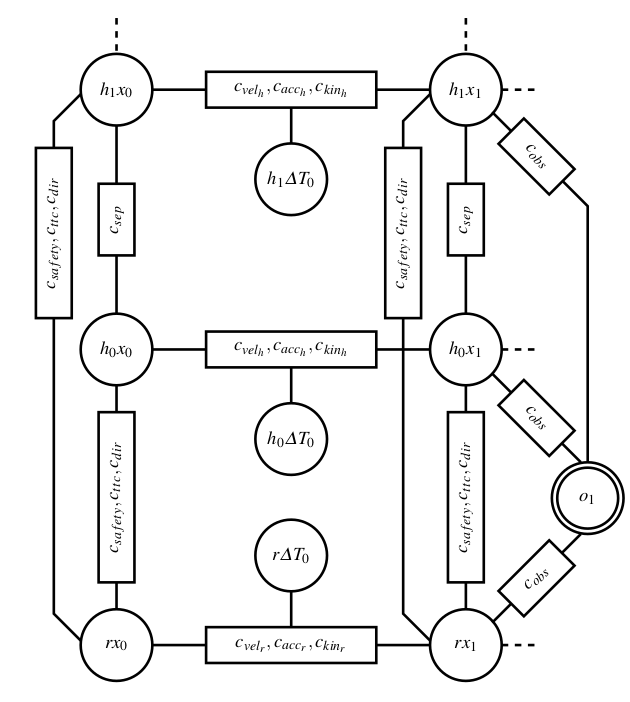
\includegraphics[width=0.9\textwidth]{figures/chapter2/hateb_graph.png}
\caption{Representation of the hypergraph being optimized from \cite{khambhaita_viewing_2017}. Simple circles represent variables to optimize (poses of agents and duration between two consecutive poses). Double circles represent fixed poses (obstacles). Rectangles are the cost functions linked to the variables they need to be computed. The total cost of the graph is computed using a weighted sum of all the constraints. This approach allows to express constraints not only on the robot trajectory ($\robotmodel$), but also on the human ones (modeling the human behaviors, $\humanmodel$) and more importantly on the interaction between the multiple agents trajectory.}
\label{fig:hateb_graph}
\end{figure}


\subsection{Constraints}
In this optimization scheme, all the constraints are represented as cost in the function. Thus, there is no \textit{hard constraints}, but using the weight of each one, we are able to prioritize some over the others. Moreover, when a trajectory has been optimized, before being executed, the local planner checks that it respects all the defined hard constraints (kinodynamic constraints and obstacles clearance).

The new formulation of Khambhaita et al. allows to separate the constaints into three categories:
\begin{itemize}
\item Robot trajectory constraints: these constraints represent the robot kinodynamic constraints (non holonomic, maximum speed, maximum acceleration) as well as preventing the robot trajectory to differ too much from the global plan. Examples are $c_{vel_{r}}$,  $c_{acc_{r}}$, $c_{kin_{r}}$ and $c_{obs}$ on Figure~\ref{fig:hateb_graph}. They are presented in \cite{rosmann_efficient_2013}.
\item Human trajectory constraints: these constraints represent the human kinodynamic constraints and prevent them to differ too much from the global trajectory. They are the same as the robot ones, but their parameters (\textit{e.g.} maximum speed threshold) must not only be set by the designer but also refined by the robot during the execution. They are represented as $c_{vel_{h}}$,  $c_{acc_{h}}$, $c_{kin_{h}}$ and $c_{obs}$ on Figure~\ref{fig:hateb_graph}.
\item Human-robot social constraints: these constraints represent how the human and robot trajectory must interact with each other. Khambhaita et al. presented the \textit{safety} constraint, ensuring a sufficient distance between the robot and the human ($c_{safety}$ on Figure~\ref{fig:hateb_graph}); the \textit{directional constraint} discouraging trajectories where the robot and the human move straight to each other ($c_{dir}$ on Figure~\ref{fig:hateb_graph}); and the \acrfull{ttc} constraint, preventing the robot and the human to adopt speed which, if maintained, would lead to a collision ($c_{ttc}$ on Figure~\ref{fig:hateb_graph}). Indeed, the idea is that trajectories containing high speeds pointing directly towards the human can increase the feeling of threat. The latter will be detailed in what follows as it was studied more in depth through a user study.
\end{itemize}

It is worth noting that different weights can be set for each constraint, and that they can be adjusted dynamically during the navigation. Moreover, by setting different weight between the robot and the human for the constraint preventing to move away from the global plan, we can adjust the \textit{stiffness} of the trajectories, thus allowing one agent or the other to elongate their trajectory, taking more or less effort into the collaborative navigation (Figure~\ref{fig:hateb_effort}).

\begin{figure}[hbtp]
\centering
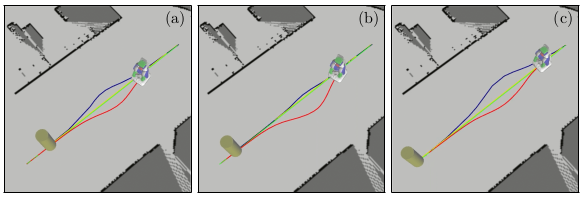
\includegraphics[width=\textwidth]{figures/chapter2/hateb_effort.png}
\caption{Different trajectory stiffnesses from \cite{khambhaita_viewing_2017}. In (a), the stiffnesses of the robot and human are set to be equal, resulting in the robot and the human altering similarly their trajectories. In (b), the robot stiffness is much lower than the human one, resulting in the robot taking most part of the effort needed to avoid the human. In rare cases, where the robot is an emergency for example, the stiffness of the human can set lower than the robot one (c).}
\label{fig:hateb_effort}
\end{figure}

In what follows we want to use this approach to study if planning for both agents can allow to make more proactive and more legible robot trajectories and if in turn this would result in a more efficient and satisfactory navigation for the human. We hypothesize that such an approach is required in intricate navigation scenarios where human and robot must cooperate to navigate successfully. This is the case in confined locations.

\section[Evaluation Through a User Study]{Evaluating Enhanced Mutual Manifestness in a Crossing Scenario}

The user study reported in this section has been made realized with Nathan Compan intern in psychology at the \acrfull{clle} laboratory (University of Toulouse Jean Jaurès), Lo\"ic Caroux associate professor in cognitive ergonomics at the \acrshort{clle} laboratory and Ophélie Carreras associate professor in cognitive psychology at the \acrshort{clle} laboratory. A journal article has been submitted and is currently under review for the \textit{IEEE Transactions on Human-Machine Systems Journal}.

In this section we present a user study aiming at assessing the pertinence of using a conavigation planner in a situation where a human and a robot must cross each other in a narrow corridor. This task of crossing in narrow corridor is challenging as both agents start in the center of either end of the corridor, and there is no way for one agent to find a way if the other agent does not move to the other side. Thus, we state that not only coplanning is required to find a plan reaching the other end of the corridor (by planning that the other agent will also cooperate and move on one side), but showing intentions and awareness of the other agent is crucial for the interaction to unfold without trouble.

\subsection{Robot Behavior Design}
For this user study we were particularly interested in finding if and how navigation coplanning would lead to higher mutual manifestness and to higher efficiency in crossing.
To do so, we designed a robot behavior using the \acrshort{hateb} navigation planner.
In their work Kambhaita et al. showed that during a narrow crossing the robot is able to plan that the human and the robot will choose opposite sides of the corridor. But if the robot shows its plan when it faces the human, they would have little time to react, and might also move to the same side as the robot, needing negotiation and replanning, reducing the overall efficiency of the crossing. The robot must thus, indicate the plan (\textit{i.e.} the planned trajectory, or here, the side of the corridor it plans to take) early enough in the crossing.

As defined in \cite{khambhaita_viewing_2017} the \acrshort{ttc} cost for two consecutive points of simultaneous points on the trajectory of the robot and the human is defined as:

\begin{equation}\label{eq:ttc}
f_{ttc}(ttc, \tau, \epsilon) = \max(0, \frac{\tau + \epsilon - ttc}{C^2})
\end{equation}
where $\tau$ is the minimum duration allowed for the time-to-collision before penalizing the configuration, $\epsilon$ is the tolerated gap between the computed $ttc$ and $\tau$ and $ttc$ is the computed duration remaining before a collision between the human and the robot if they both maintain the speed vectors they have at the considered points of the trajectories, it is infinity if no collision is computed (the cost is thus equal to 0). The complete \acrshort{ttc} cost is the addition of the all the $f_{ttc}$ for all the points on the trajectories.

\begin{figure}[hbtp]
\centering
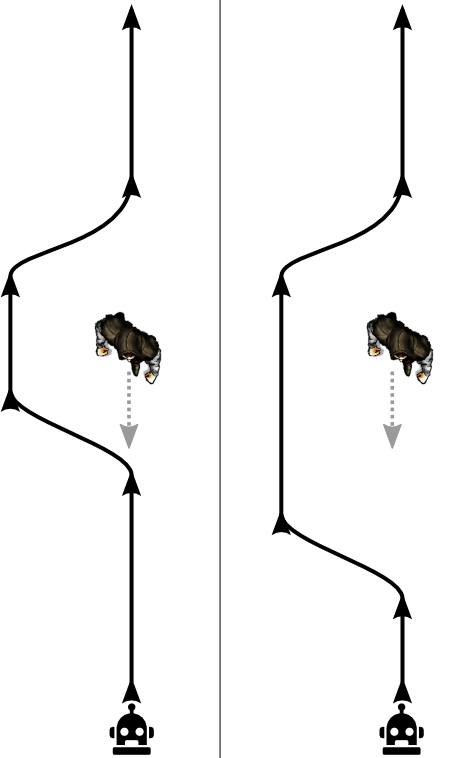
\includegraphics[scale=0.3]{figures/chapter2/condition_1_proactivity_shrink.png}
\caption{Influence of the modification of the \acrshort{ttc} constraint cost weight on the trajectory. On the left, the weight is low, the robot will show the side and avoid the human at the last moment. On the right, the weight is high, the robot will show the chosen side and avoid the human much earlier.}
\label{fig:ttc_explanations}
\end{figure}

By reducing the \acrshort{ttc} constraint function threshold and increasing its weight, we discourage trajectories where the robot and the human are facing each other at short distance or at high speed. Thus, if the robot trajectory stiffness is lower than the human one, the robot will move to the chosen side of the corridor early in the trajectory as shown in Figure~\ref{fig:ttc_explanations}.

Moreover, as stated before several papers show that using the \textit{head} of a robot can significantly improve legibility and mutual manifestness. Thus, we also chose to make the robot look at its future planned trajectory as shown in Figure~\ref{fig:head_gaze_behavior}. This is possible thanks to the \acrshort{hateb} algorithm which, unlike many other local planner only publishing  speed commands, also publishes a precise short-term trajectory. Finally, to show the robot awareness of the human presence, we made it \textit{glance} at the human twice when they enter a large and a small radius circle.

\begin{figure}[hbtp]
\centering
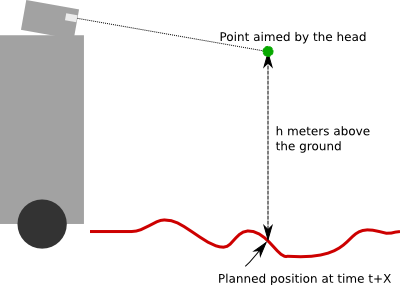
\includegraphics[scale=0.6]{figures/chapter2/head_traj_follower.png}
\caption{Behavior implemented for the robot head. The robot \textit{looks} at a point placed at its planned position X seconds in the future and h meters above the ground.}
\label{fig:head_gaze_behavior}
\end{figure}

\subsection{User Study Protocol}

\subsubsection{Objective}
The aim of this study was to evaluate the impact of the \acrshort{ttc} cost constraint and head behavior on usability. We designed a user study where actual individuals have to walk through a corridor facing a fully autonomous navigating robot. The afore-explained robot behavior was used. We measured the quality of the crossing between the robot and the human with both objective (visual behavior) and subjective data. The subjective evaluation was based on three dimensions: (1) perceived efficiency of the robot navigation, (2) user satisfaction and (3) situation awareness.

\subsubsection{Participants}
We recruited a total of 28 participants (12 males and 18 females) aging from 21 to 41 (mean: 27.32, SD: 4.13). All 28 participants had never used or interacted with a PR2 for navigation tasks, and had a neutral or good vision of robotics (mean: 5.96 over a 7 points Likert scale, SD: 1.07). This research complied with the tenets of Declaration of Helsinki \cite{world2013world}. Informed consent was obtained from each participant.

\subsubsection{Material}
A Willow Garage PR2 robot, at its lower spine position was used in this experiment. The robot measured 1.33 meters from ground to top. The entire robot can be considered as anthropomorphic and possesses a two degrees of freedom head integrating cameras resembling eyes.

The participant position was tracked using an Optitrack motion capture system\footnote{https://optitrack.com/}, tracking a worn solid headband. This system allowed the robot to track the human anywhere in the room, without looking at them.

The experiment was conducted in a L-shaped corridor (Figure~\ref{fig:experiment_adream}). The participant and the robot started from opposite side of the corridor. The participant had to walk 6 meters before entering the long straight corridor part and seeing the robot, then walk 13 meters.

\begin{figure}[hbtp]
\centering
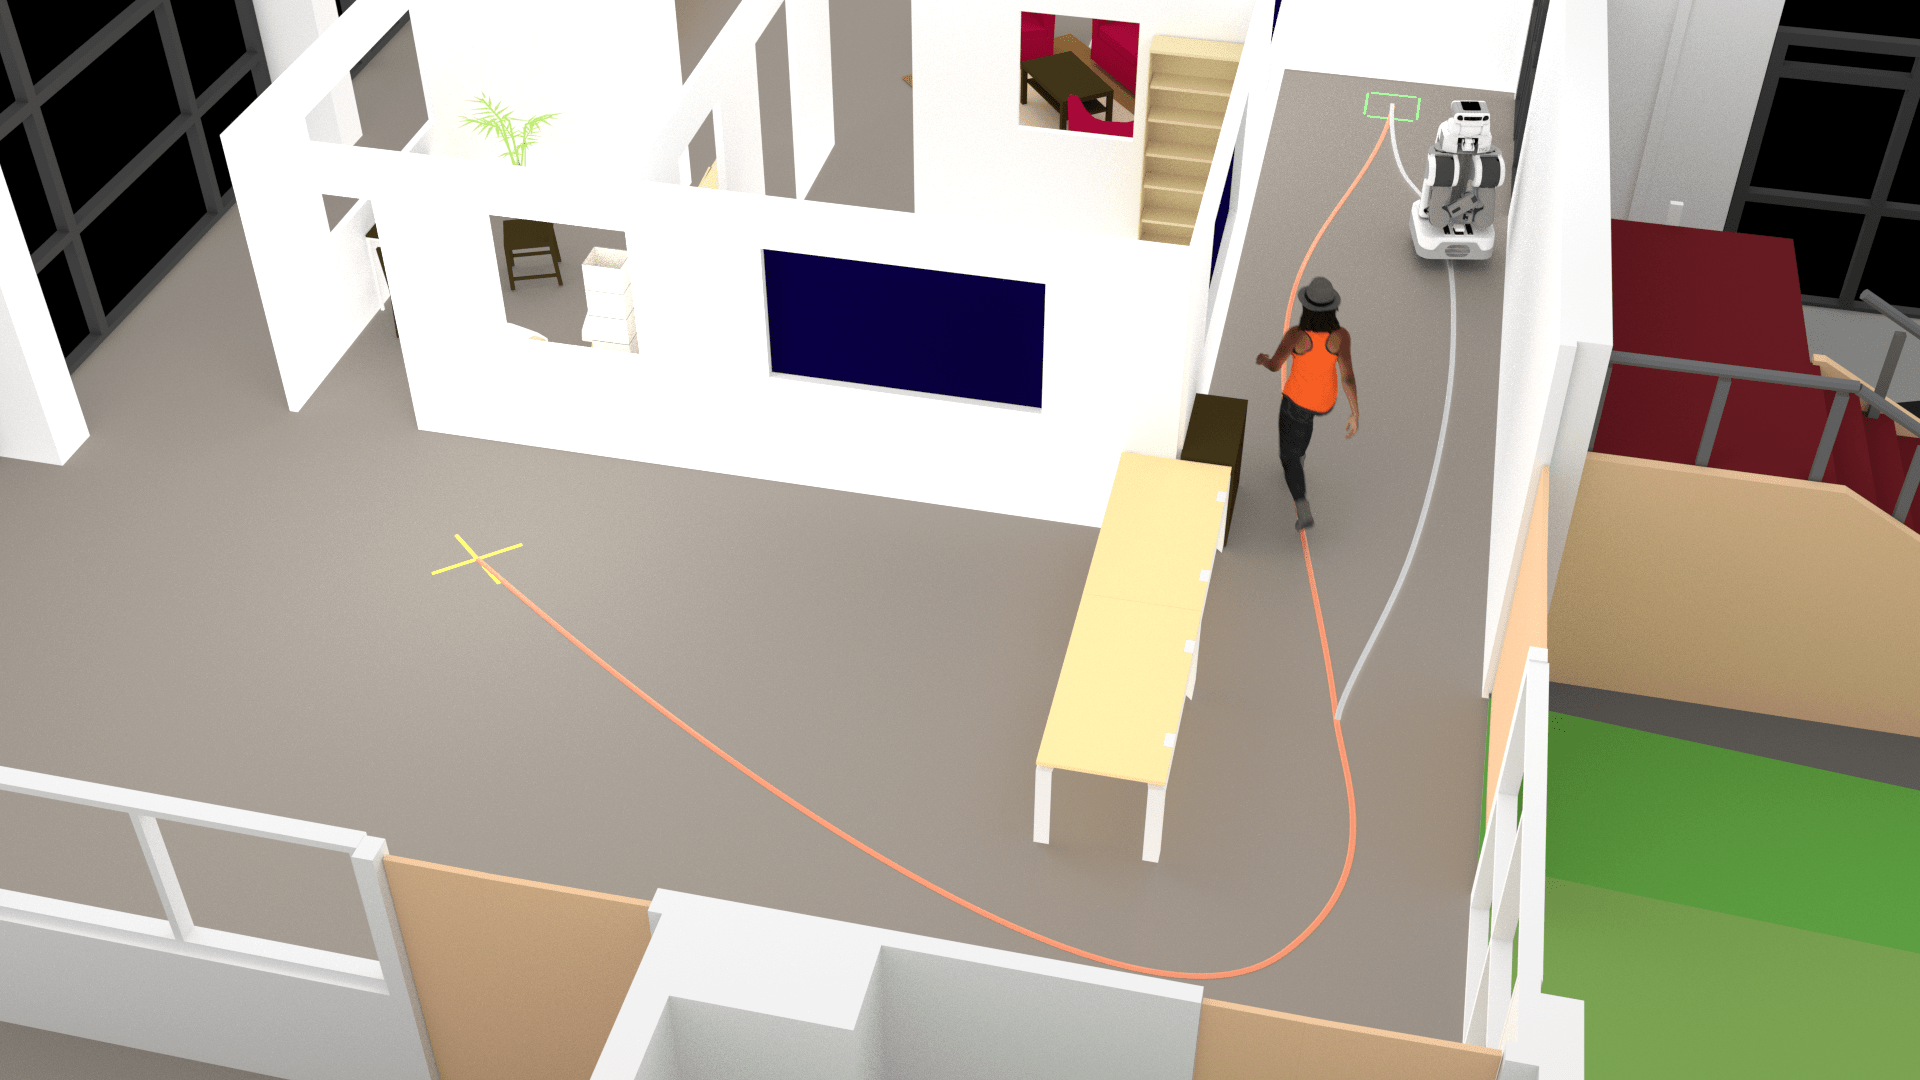
\includegraphics[width=\textwidth]{figures/chapter2/expe_human-min.png}
\caption{The  study  environment.  The  participant  had  to  go  from  the  yellow  cross  marked  on  the  ground  to  the  green  square  also  marked  on  the  ground,which was the robot starting point. Crossing occurred roughly in the area where the robot and participant are on the picture. Trajectories are displayed on the picture for example only and where not marked on the ground or suggested by the experimenters at any time.}
\label{fig:experiment_adream}
\end{figure}

We used a \textit{ETG 2w} eyetracker from SMI to collect the eye movement data of the participant. It is a portable device, allowing, after a short calibration process, to track the user gaze, and measuring where the user looks at. The data were analyzed using the \textit{BeGaze 3.6} software from SMI.

Three questionnaires and an interview were used to collect the subjective measures. They are available as submitted to the participants in French along with a proposed translation in Annex~\ref{annex:questionnaires}.
\begin{itemize}
\item Pertinence of robot decision: The \acrfull{perdita} questionnaire \cite{devin_evaluating_2018}, jointly developed between the LAAS-CNRS and the \acrshort{clle} in Toulouse, France, aims at evaluating the participant perceived pertinence of robot decision during a human robot collaborative task. In its complete form, it measures 5 dimensions: interaction, competence perception, verbal, acting and collaboration. However, in this study the robot is mute, and as the dimensions are independent we chose to remove the verbal dimension.
\item Situation Awareness: Several techniques exists to measure the situation awareness during a task \cite{endsley_design_1988}. However, they require to freeze and hide the situation to the user, and probe their working memory by questioning them about its near future. In our setup, we can't stop the robot and make it disappear while it is navigating. Thus, we have developed a series of 6 questions for measuring the user situation awareness. These questions are presented to the user just after the navigation, and ask them to rank on a 6 points Likert scale each 3 stages (2 questions per stage) of the Endsley's model: perception, comprehension and projection.
\item User satisfaction: For measuring the user satisfaction we used the AttrakDiff questionnaire. It is a standardized \acrfull{ux} questionnaire measuring both hedonic qualities and global attractiveness. We used the french translation of this questionnaire \cite{lallemand_creation_2015}.
\item Interview: The interview was constituted of 8 semi directed questions always asked in the same order. These questions aimed at qualitatively evaluating the user experience, behavior and perception of the user during the navigation. The interviewer was only allowed to read the questions and to make the participant elaborate by asking neutral questions like ``why?'' or ``can you tell me more?''.
\end{itemize}


\subsubsection{Experimental Design}
The user study was a 2 $\times$ 2 within-participants user study to evaluate how the time-to-collision constraint and the head behavior impact the robot navigation effectiveness efficiency and satisfaction. The independent variables were the \acrshort{hateb} time-to-collision cost parameters (both weight and threshold) and the head behavior. The conditions for the time-to-collision variable were $\gamma_{ttc} = 0.01$ (in Equation~\ref{eq:hateb_obj_function}) with $\tau = 1s$ (in Equation~\ref{eq:ttc})  for the \textit{low \acrshort{ttc}} condition and $\gamma_{ttc} = 15$ (in Equation~\ref{eq:hateb_obj_function}) with $\tau = 4s$ (in Equation~\ref{eq:ttc}) for the \textit{high \acrshort{ttc}} condition. For the both \textit{continuous} and \textit{alternated} head behavior conditions the robot head was pointing towards the robot planned position in 1.5s in the future at 1m above the ground. In addition, in the \textit{alternated} head behavior, the robot pointed its head towards the human when they entered the long part of the corridor during 1.5s and again during 1.2s when the robot and human were 3.5m apart. The conditions \textit{low \acrshort{ttc}} with \textit{continuous} head behavior and \textit{high \acrshort{ttc}} with \textit{alternated} head behavior are presented in Figure~\ref{fig:realttc} (a) and (b) respectively.

\begin{figure}[hbtp]
\centering
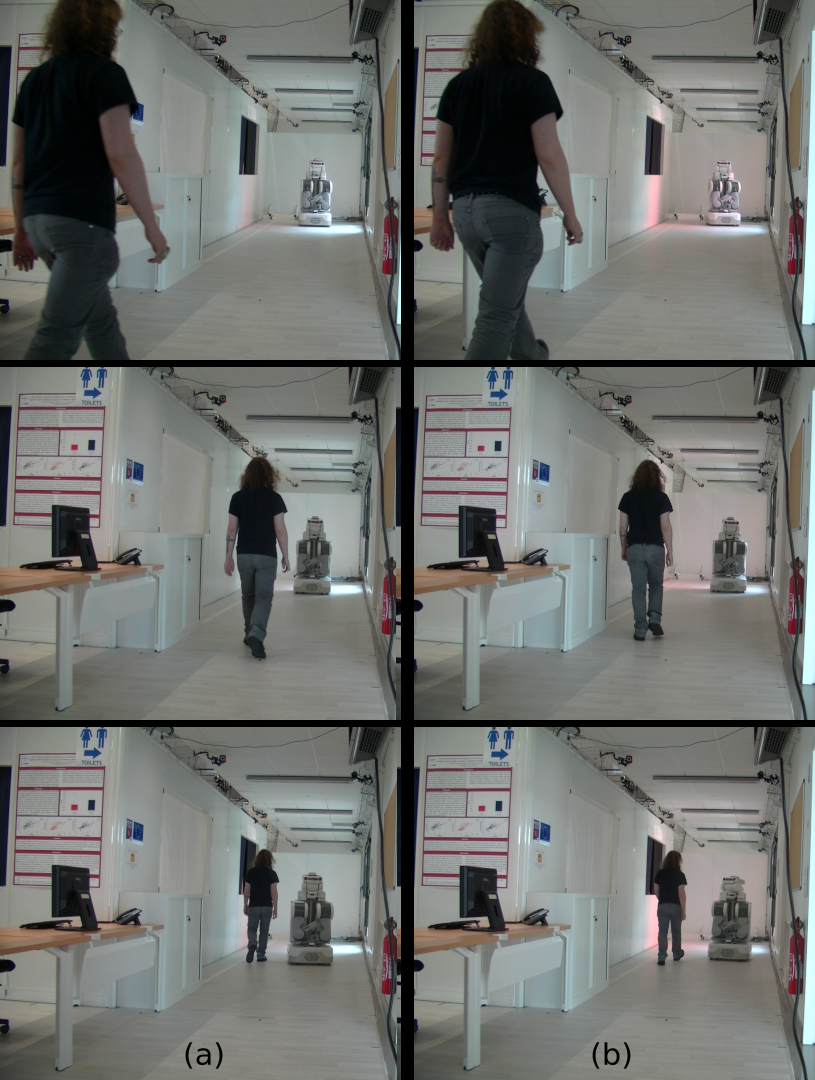
\includegraphics[width=0.95\textwidth]{figures/chapter2/Chap2ExpeReal.png}
\caption{Two typical crossings. In column (a) the robot behavior is set to the condition \textit{low \acrshort{ttc}} for the trajectory and \textit{continuous} for the head. In column (b) the conditions are \textit{high \acrshort{ttc}} for the trajectory and \textit{alternated} for the head. In (b), thanks to the \acrshort{ttc} cost, the robot starts to move to one side of the corridor very early, whereas in (a) the robot moves almost a the last moment. Moreover, in (b) the robot glances at the human when in enters the corridor, and once again when he is nearby. In (a) the robot only looks at its future position.}
\label{fig:realttc}
\end{figure}

The participant goal position was marked with a square on the ground, and was the starting point of the robot. The robot final position was 10m straight ahead of its starting position. So, the participant was able to reach their natural walking speed before turning at the corner of the L shaped corridor. The robot was only started when the participant was about to turn (2m before the turn), giving the impression that the robot was coming from further away while ensuring that the crossing happened around the same place independently of the participant walking speed.

\subsubsection{Study Procedure}
The evaluation was cut into 4 blocks. A block consisted in two same condition crossing followed by questionnaires filling. A crossing was composed by the placement of the participant and the robot on their respective starting positions, then the participant was free to go to their previously indicated goal location while crossing the robot. The three questionnaires were filled next to the participant starting location and were concerning only the two crossings made in the current block. The 4 conditions order were randomized between participants and the condition change was made between two block but never between the two crossings inside the same block.

Before starting the experiment trials, a training trial was made with the robot starting shifted to one side of the corridor and going in straight line with its head fixed looking straight. Just after this training trial, the participant was brought close to the robot and invited to inspect it. A specific head behavior was triggered making the robot head to follow the human allowing the participant to notice without being told that the robot was able to know their position and that its head could move. Moreover, the experimenter showed that robot arms were locked in place in a tucked position, and that they kept the emergency stop remote and was able to stop the robot at any time.

After the 4 blocks have been passed by the participant, the experimenter interviewed them. The audio was recorded and the answer written down.

The whole study lasted around 45 minutes per participant.

\subsubsection{Measures}
The analysis of the data was made on 27 participants because one did not fill all the questionnaires and their data were thus removed from the study. The quantitative data (questionnaires and oculometry) were analyzed using a non parametric two-way repeated measures Friedman ANOVA test.
\begin{enumerate}


\item \textit{Questionnaires}:
The three questionnaires have been passed 5 times each (one trial + four blocks). The results were codified from 1 to 7 for the \acrshort{perdita}, from 0 to 6 for the AttrakDiff and from 1 to 6 for the situation awareness questionnaire while taking care of reordering inverted items.

The \acrshort{perdita} Cronbach's alphas were for each dimension: $\alpha = 0.89$ for the interaction, $\alpha = 0.87$ for the competence, $\alpha = 0.85$ for the acting and $\alpha = 0.86$ for the collaboration.

For the situation assessment questionnaire, the Cronbach's alphas were: $\alpha = 0.93$ for the perception, $\alpha = 0.88$ for the comprehension and $\alpha = 0.87$ for the projection.

\item \textit{Oculometry}:
The oculometry data were split into two parts: before the robot crossing, and after the robot crossing (when the robot is behind the human). As we were not interested in where the participant gaze after the crossing occurred we did not analyze this part. The number and duration of fixations were measured for each of the 9 defined \acrfullpl{aoi} (Fig.~\ref{fig:aois}). The semantic gaze mapping method was used, it consists in manually selecting in which \acrshort{aoi} each automatically detected fixation lays.

\begin{figure}[hbtp]
\centering
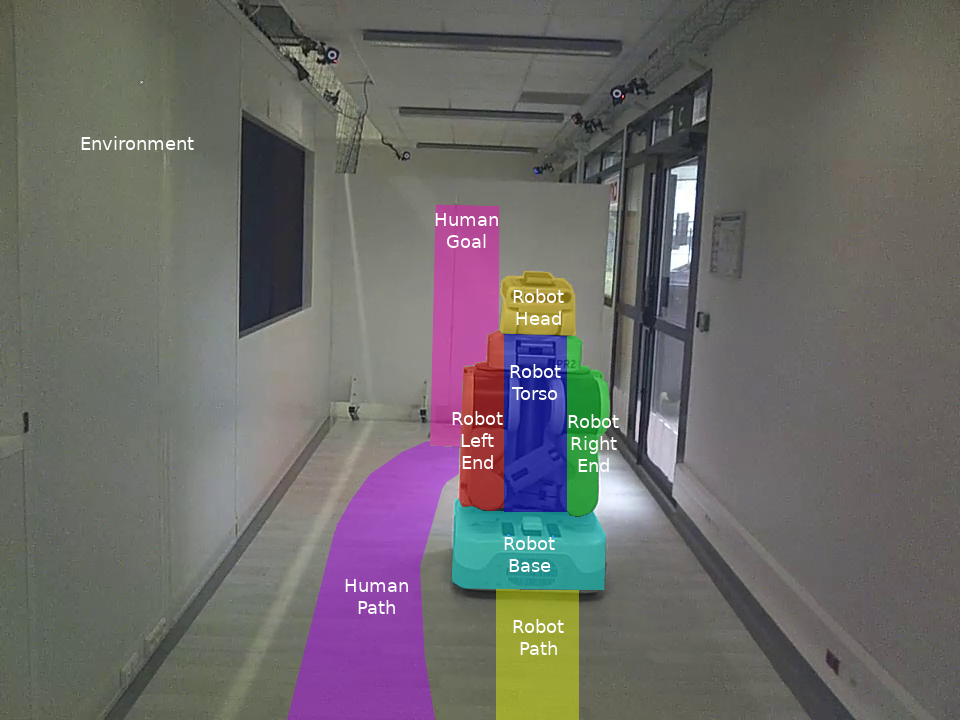
\includegraphics[scale=0.4]{figures/chapter2/pr2_aois_2.png}
\caption{The areas of interest defined to analyze the participants oculometric data.}
\label{fig:aois}
\end{figure}

\item \textit{Interview}:
The first question was a control question, ensuring that the participants saw differences between each blocks. After the second question, the interviewer revealed that the robot behavior was indeed different between each block, then proceeded to the rest of the interview. The participants answers were analyzed by excerpting verbatim (keywords or general ideas) from each question and computing their frequencies.

\item \textit{Dependent variables}:
Therefore, the dependent variables were the participant scores at the three questionnaires: \acrshort{perdita}, Situation Awareness and AttrakDiff, in addition to the number and duration of their gaze fixation during the crossing.
Prior to the experiment, the participants were asked to fill a questionnaire inquiring their age, gender, education level, profession, native language, an open question about past experience with robots and a 7 points Likert scale assessing their overall opinion about robotics.
\end{enumerate}

\subsection{Results}
\subsection{Quantitative Results}
During the crossing almost all participants (95\%) went to their left (thus, letting the robot go to their right) because the experimental setup led them to do so as the interview revealed. The robot also planned that the optimal path (given the constraints described above) was to go to the right of the human. Participants who went to their right stated they were ``testing'' the robot, thus not respecting the given goal (which was to go to the marked goal and not to test the robot). These trials have been removed from the data.

\subsubsection{Pertinence of Robot Decision In joinT Action}
The mean scores of the three dimensions of the \acrshort{perdita} questionnaire were significantly higher with an alternating head behavior than with a continuous one. The quality of interaction was higher with an alternating head behavior (\textit{M} = 5.31, \textit{SD} = 0.97), than with a continuous head behavior (\textit{M} = 5.03, \textit{SD} = 1.17), \textit{F}(1,26) = 4.41, \textit{p} < .05, $\eta_{p}^{2}$ = .15. The perceived robot competence was higher with an alternating head behavior (\textit{M} = 5.12, \textit{SD} = 1.14), than with a continuous one (\textit{M} = 4.73, \textit{SD} = 1.14), \textit{F}(1,26) = 9.15, \textit{p} < .01, $\eta_{p}^{2}$ = .26. The quality of collaboration was higher with an alternating head behavior  (\textit{M} = 5.06, \textit{SD} = 1.04), than with a continuous one (\textit{M} = 4.73, \textit{SD} = 1.14), \textit{F}(1,26) = 6.07, \textit{p} < .05, $\eta_{p}^{2}$ = .19.

There was not any significant effect of \acrshort{ttc} on the quality of interaction (\textit{F}(1,26) = 1.65, \textit{p} = .21.), on the perceived robot competence (\textit{F}(1,26) = 0.04, \textit{p} = .84), and on the quality of collaboration neither (\textit{F}(1,26) = 0.43, \textit{p} = .52). No interaction between \acrshort{ttc} and head behaviors reached significance.

\subsubsection{Attrakdiff}
The mean score of the hedonic qualities dimension was higher with an alternating head behavior (\textit{M} = 5.06, \textit{SD} = 0.87), than with a continuous one (\textit{M} = 4.93, \textit{SD} = 0,82), \textit{F}(1,26) = 4.13, \textit{p} < .05, $\eta_{p}^{2}$ = .14. There was no significant differences regarding the scores of the pragmatic qualities (\textit{F}(1,26) = 0.34, \textit{p} = .57) and attractiveness (\textit{F}(1,26) = 0.14, \textit{p} = .71) dimensions. 

There was not any significant effect of \acrshort{ttc} on hedonic qualities (\textit{F}(1,26) = 3.25, \textit{p} = .08), on pragmatic qualities (\textit{F}(1,26) = 2.97, \textit{p} = .10), and on attractiveness neither (\textit{F}(1,26) = 0.37, \textit{p} = .55). No interaction between \acrshort{ttc} and head behaviors reached significance.

\subsubsection{Situation Awareness}
The mean score of global situation awareness was significantly higher with an alternating head behavior (\textit{M} = 4.64, \textit{SD} = 0.98), than with a continuous one (\textit{M} = 4.33, \textit{SD} = 1.12), \textit{F}(1,26) = 7.77, \textit{p} < .01, $\eta_{p}^{2}$ = .23.

The mean scores of all the three dimensions of situation awareness were higher with an alternating head behavior than with a continuous one. Perception was significantly higher with an alternating head behavior (\textit{M} = 4.60, \textit{SD} = 1.08), than with a continuous one (\textit{M} = 4.15, SD = 1.29), \textit{F}(1,26) = 8.20, \textit{p} < .01, $\eta_{p}^{2}$ = .24. Comprehension was higher with an alternating head behavior (\textit{M} = 4.64, \textit{SD} = 1.05), than on a continuous one (\textit{M} = 4.36, \textit{SD} = 1.14), \textit{F}(1,26) = 5.99, \textit{p} < .05, $\eta_{p}^{2}$ = .19. Projection was higher (strong tendency) with an alternating head behavior (\textit{M} = 4.67, \textit{SD} = 0.96), than on a continuous one (\textit{M} = 4.47, \textit{SD} = 1.16), \textit{F}(1,26) = 3.52, \textit{p} = .07, $\eta_{p}^{2}$ = .12.

There was not any significant effect of the \acrshort{ttc} on global situation awareness (\textit{F}(1,26) = 1.70, \textit{p} = .20), on the perception dimension (\textit{F}(1,26) = 0.72, p = .41), and on the comprehension dimension (\textit{F}(1,26) = 0.60, \textit{p} = .45). However, the mean score of the projection dimension was higher (strong tendency) with a high \acrshort{ttc} (\textit{M} = 4.69, \textit{SD} = 0.98), than with a low \acrshort{ttc} (\textit{M} = 4.44, \textit{SD} = 1.13), \textit{F}(1,26) = 4.03, \textit{p} = .06, $\eta_{p}^{2}$ = .13. No interaction between \acrshort{ttc} and head behaviors reached significance.

\subsubsection{Gaze}
\begin{itemize}
\item  \textit{Robot vs. Environment}

The mean number of eye fixations was significantly higher on the robot (\textit{M} = 2.23, \textit{SD} = 0.98) than on the environment (\textit{M} = 1.17, \textit{SD} = 0.90), \textit{F}(1,21) = 17.82, \textit{p} < .001, $\eta_{p}^{2}$ = .46.
The mean number of eye fixations was higher (strong tendency) with a high \acrshort{ttc} (\textit{M} = 1.76, \textit{SD} =  1.04) than with a low TTC (\textit{M} = 1.65, \textit{SD} = 1.11), \textit{F}(1,21) = 3.86, \textit{p} = .06, $\eta_{p}^{2}$ = .16, regardless of the \acrshortpl{aoi}. There was not any significant effect of the robot head behavior on the mean number of eye fixations, \textit{F}(1,21) = 0.90, \textit{p} = .35. No interaction between the three factors reached significance.

The mean average duration of eye fixations was significantly higher on the robot (\textit{M} = 351, \textit{SD} =  172) than on the environment (\textit{M} = 260, \textit{SD} = 123), \textit{F}(1,18) = 6.95, \textit{p} < .05, $\eta_{p}^{2}$ = .28. There was not any other significant effects or interactions regarding the average duration of eye fixations.

\item \textit{Robot \acrshortpl{aoi}}

As shown in Table~\ref{table:eye_fixation_ttc_head}, the head was the part of the robot that was the most fixated by the participants (\textit{M} = 6.13 ; \textit{SD} = 0.59), \textit{F}(4,84) = 39.10, \textit{p} < .001, $\eta_{p}^{2}$ = .65. The number of fixations on other parts were \textit{M} = 1.28 (\textit{SD} = 0.31) for the base, \textit{M} = 1.16 (\textit{SD} = 0.23) for the torso, \textit{M} = 0.95 (\textit{SD} = 0.19) for the right end, and \textit{M} = 1.64 (\textit{SD} = 0.37) for the left end. 

\begin{table}[!htbp]
	\centering
    \begin{tabular}{lcccc}
    \hline
    \multirow{2}{*}{\textbf{Robot AoI}} & \multicolumn{2}{c}{\textbf{Low TTC}} & \multicolumn{2}{c}{\textbf{High TTC}} \\
    \cline{2-5} 
               & \textbf{Continuous}  & \textbf{Alternating}  & \textbf{Continuous}  & \textbf{Alternating}   \\
    \hline
    Head       & 5.64 (3.42)  & 5.50 (2.78)  & 5.93 (2.90)  & 7.45 (3.80)   \\
    Torso      & 1.39 (1.39)  & 1.14 (1.49)  & 1.39 (1.65)  & 0.73 (0.96)   \\
    Left end   & 0.95 (1.20)  & 1.07 (1.11)  & 1.00 (1.15)  & 0.77 (1.14)   \\
    Right end  & 1.82 (1.92)  & 1.55 (1.71)  & 1.55 (1.94)  & 1.64 (2.27)   \\
    Base       & 1.36 (2.07)  & 1.23 (1.53)  & 1.45 (1.65)  & 1.07 (1.27)   \\
    \hline
\end{tabular}
   \caption{\label{table:eye_fixation_ttc_head} Mean number of eye fixations made by participants in each \acrfull{aoi} of the robot in each experimental condition (\acrshort{ttc} x robot head behavior) in main experiment. Standard deviations are shown in parentheses.}
\end{table}

There was a significant interaction between the \acrshort{aoi} type and the type of \acrshort{ttc}, \textit{F}(4,84) = 5.72, \textit{p} < .001, $\eta_{p}^{2}$ = .21. The robot head was more fixated when the \acrshort{ttc} was high (\textit{M} = 6.69, \textit{SD} = 3.43) than when it was low (\textit{M} = 5.57, \textit{SD} = 3.08). There was an interaction (strong tendency) between the \acrshort{aoi} type and head behaviors, \textit{F}(4,84) = 2.34, \textit{p} = .06, $\eta_{p}^{2}$ = .10. The robot head was more fixated, when the robot head was alternating  (\textit{M} = 6.48, \textit{SD} = 3.43) than when it was continuous (\textit{M} = 5.78, \textit{SD} = 3.14).

In addition, there was a double interaction (strong tendency) between the \acrshort{aoi} type, head behaviors and the type of \acrshort{ttc}, \textit{F}(4,84) = 2.41, \textit{p} = .06, $\eta_{p}^{2}$ = .10. Table~\ref{table:eye_fixation_ttc_head} shows that the robot head was more fixated when the robot head was alternating only with a high \acrshort{ttc}.

There was not any significant effect of the robot head behaviors on the mean number of eye fixations, \textit{F}(1,21) = 0.13, \textit{p} = .73. There was not any significant effect of the \acrshort{ttc} type on the mean number of eye fixations, \textit{F}(1,21) = 1.82, \textit{p} = .19. The interaction between the TTC and the head behaviors, \textit{F}(1,21) = 0.74, \textit{p} = .40, did not reach significance.

The ANOVA for the mean duration of eye fixations was not possible due to an absence of data in some experimental conditions.
\end{itemize}

\subsection{Qualitative Results}
All the participants saw differences between blocks, 19 of them saw head behavior differences and 10 of them saw trajectory differences. When the participant talked about the alternated head behavior, positive adjectives were employed (``reassuring'', ``sympathetic'', ``interactive''\footnote{``sécurisant'', ``sympathique'', ``interactif'' in French}), when they talked about the continuous head behavior, negative adjectives were employed (``unsettling''\footnote{``troublant'' in French}).

After the experimenter revealed that the robot behavior was different in each block, the participants preferred when the robot was ``moving its head'' (12 participants). Five participants also preferred when the robot changes its direction long before they cross. Participants did not appreciate when the robot kept a ``fixed head'' because they thought the robot was not aware of them (8 participants), when the robot was ``hesitating'' (4 participants) and when it came ``too close'' (4 participants).

Fourteen participants found the robot was the most competent in the condition with the alternated head behavior and high \acrshort{ttc}, because the robot became aware of them when looking at them (10 participants), because the robot changed its direction sooner (4 participants), because it was trying to avoid them (4 participants) or because it was not coming too close (3 participants).

The participants found the robot more acceptable when it made a ``visual contact'' (4 participants) and when it changed its trajectory early (3 participants). They found the robot less acceptable when the robot came too close (6 participants), when hesitating (3 participants), when not making visual contact (2 participants).


\subsection{Discussion}
This study aimed at exploring how taking into account the human model and planning for both human and robot during navigation allows to easily design behavior enhancing the usability of the robot. More precisely, navigation coplanning allows to easily implement coordination smoothers and increase mutual manifestness, we thus hypothesized that these changes should lead to a significant impact on robot usability in the intricate scenario of narrow corridor crossing.

Human gaze analysis showed that head of the robot was fixed many times and even more when the robot showed its chosen corridor side early in the navigation (with a high \acrshort{ttc}). Moreover, subjective results revealed that moving the head of the robot in an alternating pattern (pointing towards its path while sometimes pointing at the human head) improved the perception of the quality of interaction, the perceived robot competence, and the quality of collaboration. This alternative head behavior also increases the situation awareness score. \textbf{This strongly support previous results on using the robot head during human robot navigation scenarios} \cite{khambhaita_head-body_2016}, \cite{may_show_2015}.

However, the satisfaction seems to have been slightly improved (on hedonic quality) when the robot presented the alternating gaze behavior rather than the continuous one. This result is only a tendency, but in the interview, the participants identified as positive when the robot moved its head to glance at them and changed its trajectory. They also identified as negative when the robot was too close or did not look at them. We think these discrepancies between the AttrakDiff results and the interview are caused by our poor questionnaire choice. Indeed, the AttrakDiff questionnaire aims at measuring the satisfaction produced by a final product (\textit{e.g.} cellphones) and the willingness of a user to buy this product, but not the satisfaction of a user when dynamically interacting with a robot in a navigation scenario. Yet, as no other questionnaire to our knowledge proposed to measure user satisfaction during human robot interaction, we chose the AttrakDiff.

Results show that using the \acrshort{hateb} navigation co-planner with a high time-to-collision weight constraint cost and low threshold, alongside an head behavior signaling future robot trajectory and the human awareness during a crossing in a constrained space allows the human to have a better situation awareness and to perceive the robot as acting more pertinently and being more competent. \textbf{This finding supports the result from Lu et al.} \cite{lu_towards_2013}, where the navigation efficiency is increased when the robot looks at the human and shows a ``social'' navigation behavior.

We speculate that both the high \acrshort{ttc} and alternating gaze of the robot are needed to improve the interaction and that no simple effect are significant for multiple reasons. First, with only the robot choosing a corridor side early in the crossing (high \acrshort{ttc} condition) without showing the human awareness (continuous head condition), it may not be obvious to the human that the trajectory change is due to their presence. Conversely, when the robot signals its awareness of the human (here by pointing its head towards them) but without taking any action to ease the interaction (low \acrshort{ttc} condition), the human stays in a situation where they don't know what the robot will do next. Finally, by both making the robot show its human awareness and change its own trajectory to facilitate the interaction (coordination smoother), it becomes clear the that robot is proposing a co-navigation solution where both agents are avoiding each other.

Finally, oculometry results indicate that when the head is recognized as an information provider (in the alternating head condition), information are most likely to be sought in the robot head motion. The head is also looked longer when the robot alternately looks at the human. We can also note that people tend to think PR2 is getting data through its head, probably because of the visible cameras on it, even when it is not the case (like in our experiment).

\improvement{Ajouter limites et future works de l'étude ? Ou le mettre dans la section conclusion ?}

\section{On User Studies in HRI}
After doing this user study, we wanted to report the experience and to discuss it with the community. Thus, we decided with a PhD student in psychology, Kathleen Belhassein, to participate to a workshop at HRI 2019 entitled \textit{Test Methods and Metrics for Effective \acrshort{hri}}. It seemed interesting to collaborate to have two points of view on user studies, coming from psychology for her, and from \acrshort{hci} and \acrshort{hri} for us. We identified three main challenges concerning user studies in \acrshort{hri}: the users, the evaluation methods and the replication. We concluded by presenting ten recommendations for user studies in HRI \cite{belhassein2019towards}. According to the discussion with the community during the workshop, we updated and submitted a contribution, which has been accepted, to the \textit{Transactions on Human-Robot Interaction} journal.

\subsection{Users in HRI studies}
When conducting a user study, we obviously recruit today's users, with their past experiences and expectations with robotics. Kuhnert et al. showed the existence of a \textit{gap} between the user's attitude towards existing robots and their expectations about the  ideal everyday social robot \cite{kuhnert2017gap}. Thus, when evaluating a human robot interaction it is important to evaluate the three aspects defined by Desmet and Hekkert: the instrumental interaction (interaction for expected purpose: always evaluated in current user study), the non-instrumental interaction (interacting for other than main purpose: often non evaluated) and the non-physical interaction (expectations: often under evaluated) \cite{desmet2007framework}. Indeed, non-physical interaction refers to all preconceptions of the robot by the user, they could come from past experiences or imagination. Since today's users have almost no past experiences with robot, those anticipations come mainly from imagination and fantasies and can widely vary from one to another. Thus, it is really important to evaluate the mindset of the user before the study. Some tools used in psychology can be useful in this context. For example, the implicit association test \cite{greenwald1998measuring}, used to measure automatic and implicit associations like prejudices, or priming paradigms could be used to control the expectations and beliefs of subjects towards robots.

Moreover, as many of the recruited users has none to very few past experiences with robots, the novelty (and wouaw) effect when interacting with robot during a one shot study is huge, and may not be representative of a robot long term use. To assess this \textit{cumulative experience}, \acrfull{ux} and \acrfull{hci} designers conduct \textit{longitudinal studies} \cite{lazar2017research}, gathering data on a long period of time. However, in the human-robot interaction field, this study may not be applicable as is. Indeed, the used material (robots) is expensive and often in limited quantities in laboratories. In order to diminish this effect, the evaluation should be part of a larger, more cognitively intense or time pressurizing task where the user must almost \textit{forget} about everything concerning the robot except the part to be evaluated, which should be crucial in this task. This effect could also be reduced by making an habituation phase at the beginning of the experiment, in which the user can act more freely with the robot.

In some \acrshort{hri} studies, a questionnaire is administered before the interaction task in order to apprehend the degree of familiarity and knowledge of the participants about the robots. Even if some recruited people are from the same professional environment and are therefore already accustomed to robots, this measure of knowledge about robots is never used to remove participants from the user study. In addition to the bias that this recruitment may pose, the sample is therefore not representative of the general population but of a particular subpopulation. To ensure a better representation of the population, it would therefore be necessary to randomly sample and recruit outside of the professional circle.

Finally, \acrshort{hri} studies have frequently few participants. For example, about 44\% of user studies published in the proceedings of the conference HRI'17 involve fewer than 30 participants. However, the size of the sample is a prerequisite for obtaining sufficient statistical power to conclude on the results obtained, and to avoid type I errors (false positive) or type II (false negative). Beyond the statistical issues, it seems important to be modest about the conclusions drawn from studies involving too few participants, and therefore not to generalize to the population the results obtained.

\subsection*{The Particular Case of Web Studies}

To respond to this difficulty and have a large number of participants, it is now frequent to be confronted to web studies (as in \cite{khambhaita_head-body_2016}), especially via the crowdsourcing web platform Amazon Mechanical Turk. Indeed, it is then much easier to recruit participants and have them take small tasks or questionnaires directly online. It seems however important to be vigilant on the study conclusions, since we are not in a context of human-robot interaction in its strictest sense; the participant is not confronted to the robot, does not share its physical space, and therefore will not have the same reactions that he would have during an interaction in the real world. Nevertheless, it could be an interesting tool for participatory design studies, \textit{i.e.} all the studies that do not deal with a fully implemented robot that must be evaluated but rather that serve to explore the responses of users to certain specific behaviors and to collect their opinion. 

\section{Evaluation Methods}
\label{sec:evaluation}

The key concept in \acrshort{hci} is usability, which regroups effectiveness (ability to perform a task), efficiency (ability to perform the task without wasting resources) and satisfaction. More often than not, \acrshort{hri} user studies focus on user satisfaction (and \textit{acceptability}) evaluated with questionnaires created or adapted specifically for this context of interaction or borrowed from \acrshort{hci}. Even if \acrshort{hri} studies join the field of Human-Computer Interaction and user experience design by the fact that they are both trying to improve the human use of interactive systems, it is a hugely different experience to interact either with a robot or a computer. We must not forget that in the case of \acrshort{hri} studies, there are two agents that interact and no longer an agent that interacts with a product/an interface. Therefore, the methods and tools of \acrshort{hci} are not always suitable to be used during a situation of interaction between a human agent and a robotic agent. First of all, people tend to attribute mental states and human traits to robots. This human tendency to anthropomorphism is not only dedicated to robots but also animals, objects or natural phenomenon. However, robots are more perceived as an agent endowed with lifelike qualities than other technologies. 
In addition, the perceived risks to evolve in the same environment as a robot are obviously not the same than when we use computers or other technologies, and can induce negative emotions or feeling of insecurity \cite{dautenhahn2006may}. 
Thus, these particularities in the subjective experience of interacting with a robot has to be considered in the build of experimental and evaluation tools.

\subsection{Use of Self-Assessment Methods}

Although the simplest and most widespread evaluation method in HRI studies is the self-assessment method with questionnaires, it is necessary to understand that there may be a significant difference between what subjects self-report of their own experience and what they really experienced and felt, for example because of the social desirability bias \cite{fisher1993social}. In addition, there are very few questionnaires created for \acrshort{hri} studies that meet the validity and standardization criteria of these methods. Indeed to be validated, a questionnaire must be reliable and consistent, \textit{i.e.} the results must be replicate in comparable situations; it must be valid, that is to say it actually measures what it is supposed to and not another dimension; and finally, it must be sensitive to change. More often than not, HRI questionnaires are simply evaluated on their internal consistency (all the items from one dimension are correlated to each other) with Cronbach's alpha. However, to valid that the questionnaire measures the construct of interest, it would be important to use on a pilot study another method of evaluation for this same construct and use correlation matrices between them \cite{tsang2017guidelines}. 

Finally, it is common to see questionnaires used in another language. However, if a questionnaire is created in a specific language it has to be used only in that language. It is therefore absolutely necessary when using a questionnaire from another language to use the back translation method (\textit{i.e.} translate back into the original language the questionnaire previously translated into the target language). In addition, the questionnaire once translated must imperatively be validated following the same rules as an original questionnaire, to ensure that the translated version measure the exact same construct at the original, as it was the case for example for the French translation of the \acrshort{ux} questionnaire AttrakDiff \cite{lallemand_creation_2015}.

\subsection{Other Evaluation Methods for Acceptability}

Including heart rates, brain or skeletal muscles electrical activity, blood pressure, respiratory frequency or even galvanic skin responses, there are a number of different physiological measures that can be used to evaluate the participant's physiological response in touch with a robot. These evaluation methods have the advantage of being able to prevent participants from consciously modifying their answers, as this is the case with self-assessment measures.

In interaction situations and even more in cooperative situations, taking social signals into account may also be useful for assessing the human ability to accept to engage into a task with a robotic partner. Behavior observation techniques are for example used to measure shared gazes, in particular with video recording and eye tracking \cite{gharbi2015toward}.

\subsection{Evaluate Efficiency and Effectiveness in Human-Robot Interaction}
But what is the point of making a robot behavior satisfying but useless? 
Once more, tools exist in \acrshort{hci} to measure the other components of usability but are not always adapted to \acrshort{hri} studies. For example, freeze-probe techniques are frequently used in the case of evaluating the situation awareness (\textit{i.e.} the perception, comprehension and projection of elements in the environment \cite{endsley_design_1988}). They consist of freezing the task in progress and administrating a questionnaire about the situation at the exact moment of the freeze point \cite{salmon2006situation}. Such a device, mostly developed for use in the aviation or military domain, is a real challenge and almost impossible to apply in \acrshort{hri}, since we are in the case of a real-world physical interaction with a robotic agent and we can not just make the robot disappear.

Most of the existing \acrshort{hri} questionnaires deal more with the physical aspect of the robot and its acceptability by the user (\textit{e.g.} the godspeed questionnaire~\cite{bartneck2009measurement} and the RoSAS questionnaire~\cite{carpinella2017robotic}) than its effectiveness and usefulness.
In previous work, we tried to propose a preliminary version of a questionnaire specific to \acrshort{hri} studies and measuring the decision-making processes of the robot in a joint action context with a human~ \cite{devin_evaluating_2018}, but this tool remains at the draft stage and deserves to be refined, coupled with other evaluation methods, used in other studies and finally validated according to the criteria of self-assessment methods.

Moreover, adding efficiency/effectiveness measurements in a study can be pretty simple given the technical abilities inherent to robots (\textit{e.g.} timing the task completion, the number of user errors). Thus, we could consider using the robot as a tool for measuring its impact on the human performance, and therefore evaluate the efficiency of human-robot interaction. Mayiama \textit{et al.} presented several metrics, and implemented some of them in a robotic component, to evaluate in real-time the \textit{quality of interaction}. These data can also be analyzed more deeply afterwards to evaluate the interaction. In addition, one of the most widely used methods of cognitive psychology is mental chronometry, which uses reaction times as a measure, and refers to the temporal study of information processing \cite{posner1978chronometric}.

Whether it concerns the evaluation of acceptability or efficiency and effectiveness in human-robot interactions, a more frequent use of objective measures (\textit{e.g.} physiological or task performance measures) could improve the validity of the results of \acrshort{hri} studies and their methodological rigor. These different techniques must still be consistent with each other in their use in a user study, this recommendation is not always feasible but should be taken into account when establishing the methodological plan.

\section{The Replication Crisis in HRI}
\label{sec:replication}

Replication of results is an important concept for any discipline following the scientific approach; it is a question of repeating a study to determine if the results are reproducible and therefore reliable. Psychology and more generally social and medical sciences have known since the 2000s what is called the replication crisis.
Indeed, if the replication crisis begins to appear in \acrshort{hci} \cite{echtler2018open} mainly because of closed source code used in the experiments, \acrshort{hri} presents other issues. First, the code used in robotic studies is often much more complex and heavy to use. Indeed, to evaluate a high-level component (\textit{e.g.} a task co-planning algorithm) a whole component stack is needed (\textit{e.g.} low-level motor controllers, path finding, trajectory following, motion planning, localization, face detection, speech synthesis, speech recognition). If some of those components are standards and widely available, others can be state of the art, unstable or even tweaked by the experimenters to match their own needs, making it more difficult to replicate the experiment if those components are not precisely described or not available. Moreover, the material used can also be changed (\textit{e.g.} by 3D printing a gripper to fit the object manipulation task needed), and components tuned to work accordingly. Those small changes on the hardware and on the software needs to be reported, else the experiment replication is impossible.

Finally, many user studies in \acrshort{hri} used Wizard of Oz technique, because robotic systems are often not robust enough to act autonomously in an environment with humans. The use of Wizard of Oz technique makes very difficult the exact replication of the situation due to the fact that the complete scenario of the study is not available. 
In the case of \acrshort{hri} evaluation, we can also ask ourselves if humans evaluate the robot or the human controlling the robot.

\subsection{Proposed Guidelines for Better User Studies in HRI}
By taking all those issues and solutions coming from different fields we might provide some checkpoints when designing a \acrshort{hri} user study:
\begin{enumerate}
    \item The \textit{more users} the better. It improves the statistic analysis of the study and could erase some bias.
    \item \textit{Widen} the recruitment. Your colleagues know a lot about technology: randomly recruit people in your bakery, in the supermarket, using flyers...
    \item \textit{Be rigorous} with your protocol. There are so many unwanted uncontrolled variables. Don't be one!
    \item Let the user \textit{accustom} to the robot and its behavior before starting the experiment. In order to diminish the ``wouaw'' effect and make measures closer to a long term use.
    \item Make sure your experiment is physically and psychologically \textit{safe}. Apart from hurting a user, you risk to prevaricate your measures if the experimenter is stressed about something going wrong.
    \item Objectively \textit{measure if your robot is useful} in what you are making it do. A robot can be really satisfying, but it will be quickly forgotten if it does nothing.
    \item Use the \textit{right tools} for your measurements. Widely used and standardized tools will give more credibility to your study. Questionnaires are not the end.
    \item Make theoretically solid and valid \textit{tools} specific to \acrshort{hri} and publish them if they don't exist. It will benefit the whole community.
    \item \textit{Give as much details as possible} about your study. Gives the source code, hardware schematics or references and the description of the environment in order to make others able to reproduce your experiment.
    \item When doing a \textit{Wizard of Oz be rigorous}. Emulate only a small, non-evaluated, component of your robot. Write the rules you follow down, respect them and publish them along with your study.
\end{enumerate}

\section{Extending HATEB}
Closing this general parenthesis about user studies in \acrshort{hri}, we continue on the \acrshort{hateb} navigation planner development. Having shown that providing co-navigation solution using \acrshort{hateb} can effectively be used to enhance the efficiency of the interaction, we will present in this section the different extensions made to \acrshort{hateb}.

\subsection{Adapting HATEB to Other Robots}
Khambhaita et al. \cite{khambhaita_head-body_2016} successfully used \acrshort{hateb} on a PR2 robot, both in simulation and on the real platform. As the approach is general, we implemented it on other robots.

\subsubsection{Using HATEB on a Legged Humanoid Robot}
Legged humanoid robots are characterized by their bipedal navigation, tremendously increasing the complexity of navigation and control with regards to wheeled robots. However, legged robots present a large advantage for social and human robot interaction as human infrastructure are often thought for being navigated with legs rather than with wheels. Thus, we tried to implement our approach to a humanoid robot.

To do so, we partnered with the Gepetto team at LAAS-CNRS specialized in humanoid systems motion. Thanks to their modular software architecture presented in \cite{stasse_modular_architecture_2008}, only minor changes had to be done to \acrshort{hateb} to integrate with their other components.

One of their component \cite{naveau_reactive_walking_2017} takes as parameter a (simplified) robot kinematic model and is able, in real-time and at typical joint position control frequencies (around 200~Hz), to give position command to all the robot joints in order for the center of mass of the robot to respect a speed command given as input. Thus, we can generate a non-holonomic trajectory for the robot with \acrshort{hateb} and send the returned speed commands to this component. Given a speed command, the component is able to generate footstep placements and to compute robot joint positions ensuring the equilibrium and the respect of the kinodynamic constraints (between two successive poses) of the robot. However, this component has no ROS interface whereas \acrshort{hateb} is heavily built for ROS use. Thus, we made a bridge transferring the speed commands output by \acrshort{hateb} to the Gepetto architecture and transferring back the joint position commands.

This has only be run virtually, and for simplicity, no simulator was used. Instead, we assumed the joint position command to be immediately and perfectly executed. Such an assumption has been made possible because of the effectiveness of the Gepetto architecture, having a tested precise model of the robot, ensures that the kinodynamic constraints will be respected, and consequently gives a correct robot behavior.

We tested this approach on a virtual HRP2 robot, with a virtual human (Figure~\ref{fig:approach}). We were able to make the robot avoid the human in a face to face crossing, while accounting also for the human ability to avoid the robot. Moreover, using this approach is pertinent as HRP2 has much slower dynamics than PR2, and thus must rely a lot on the ability of the human to avoid it. Indeed, if the robot maximum speed or acceleration parameters were set too high in \acrshort{hateb}, the speed commands generated would make the robot fall. Planning for both the human and the robot allows to generate smoother avoiding trajectories for the robot by assuming the human can take most of the effort. 

\begin{figure}[hbtp]
\centering
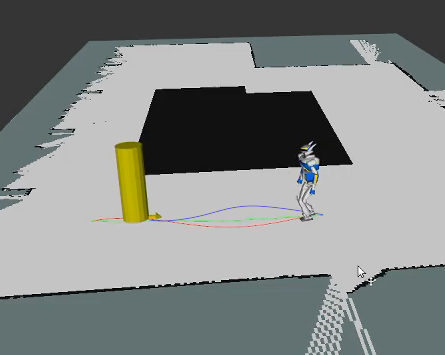
\includegraphics[width=0.6\textwidth]{figures/chapter2/Chap2HRP2.png}
\caption{The trajectory generated for the human and HRP2 in simulation. The green trajectory is the global plan initializing the optimizer. While the red trajectory (robot) is smooth and make a wide turn, the blue trajectory (human) is planned to be turn sharper and to take more effort in the crossing. Indeed, the robot model was set with slower dynamics (small maximum speed and acceleration) than the human model as HRP2 must move slowly not to fall.}
\label{fig:hrp2}
\end{figure}

However, using \acrshort{hateb} we constraining even more the motion of the legged robot. Indeed, the presented version of \acrshort{hateb} does not support holonomic trajectories, which would be doable by PR2 and HRP2. Using this approach, HRP2 cannot make a step on the side, but has to turn and move forward. The current version of \acrshort{hateb} now integrates holonomic capabilities thanks to Phani-Teja Singamaneni \cite{singamaneni2020hateb}, but has not be integrated for the HRP2 robot yet.	

This preliminary work not only shows the versatility of the approach, but also that planning for both can be useful for a constrained robot. Indeed, with a slow dynamic robot, a classical navigation planner may find no solution to avoid an approaching human, but by planning that the human can make a great effort to avoid the robot, it can generate a trajectory for the robot that elicit a plan for the human to follow.

\subsubsection{An Experiment With the Pepper Robot for Close Human Robot Motions}
The European project \acrshort{mummer}\footnote{\url{http://mummer-project.eu/}} aimed at deploying a Pepper robot in a shopping mall in Finland to entertain and guide customers \cite{foster2019mummer}. The project regrouped seven different stakeholders bringing their knowledge to the project. The LAAS-CNRS goal was to make the guide task. However, in order to serve the most customers possible and to cope with large navigation issues of the Pepper platform, we choose not to go with the customer all the way to the asked shop, but instead, as the mall employees usually do, give directions to the customer to help them find the requested shop. We call this more precise task \textit{route description}.
However, giving only verbal instructions concerning the route is not sufficient, we chose to make the robot point the shop, if it is visible from the current position, or point its direction and the first visible element of the route otherwise.

Although, the surroundings of the robot home place (the place in the mall where the robot is located, and thus, where the interaction takes place) contains some obstacles such as barriers, structure poles and advertisement posters. Thus, the object the robot has to point to the human might not be visible from their current position. We thus endowed the robot with the ability to compute the optimal position for the human and the robot for it to point at a landmark. This computation details can be found in \cite{waldhart_reasoning_shared_2019}. Once the robot has computed these optimal positions, it needs to move to its one while ensuring the human can move to theirs. Moreover, the customers might be hesitant to approach the robot to start an interaction, thus, the robot is also able to approach a nearby human to ask them if they need its help. However, it has to consider that the human might also move towards the robot to encounter it.

To tackle both of these issues, we decided to use \acrshort{hateb}. We made a higher level component proposing three services: rotate, navigate to and approach. While the rotate service is only made for in place rotation of the robot in order to reorient itself for repositioning or to look or point at something, the other two uses the \acrshort{hateb} planner described earlier. The navigate to service expects a robot goal pose and optionally a human identifier and a human goal (which is shown by the robot before starting the navigation). The \acrshort{hateb} planner is then called with empirically tuned weights to make the robot navigate to its goal position while, if provided, ensuring the human can reach theirs. The approach service expects a human identifier and a distance, and use the \acrshort{hateb} planner with different weights with a goal at the specified distance in front of the human. The human goal is predicted from their current pose and velocity some seconds in the future, and updated at each control loop with their new sensed pose and speed.

Moreover, by using \acrshort{hateb}, we were able to use the same head behavior as the one described in Figure~\ref{fig:head_gaze_behavior}, aiming at improving the legibility of robot motion, crucial in such close motions.

\begin{figure}[hbtp]
\centering
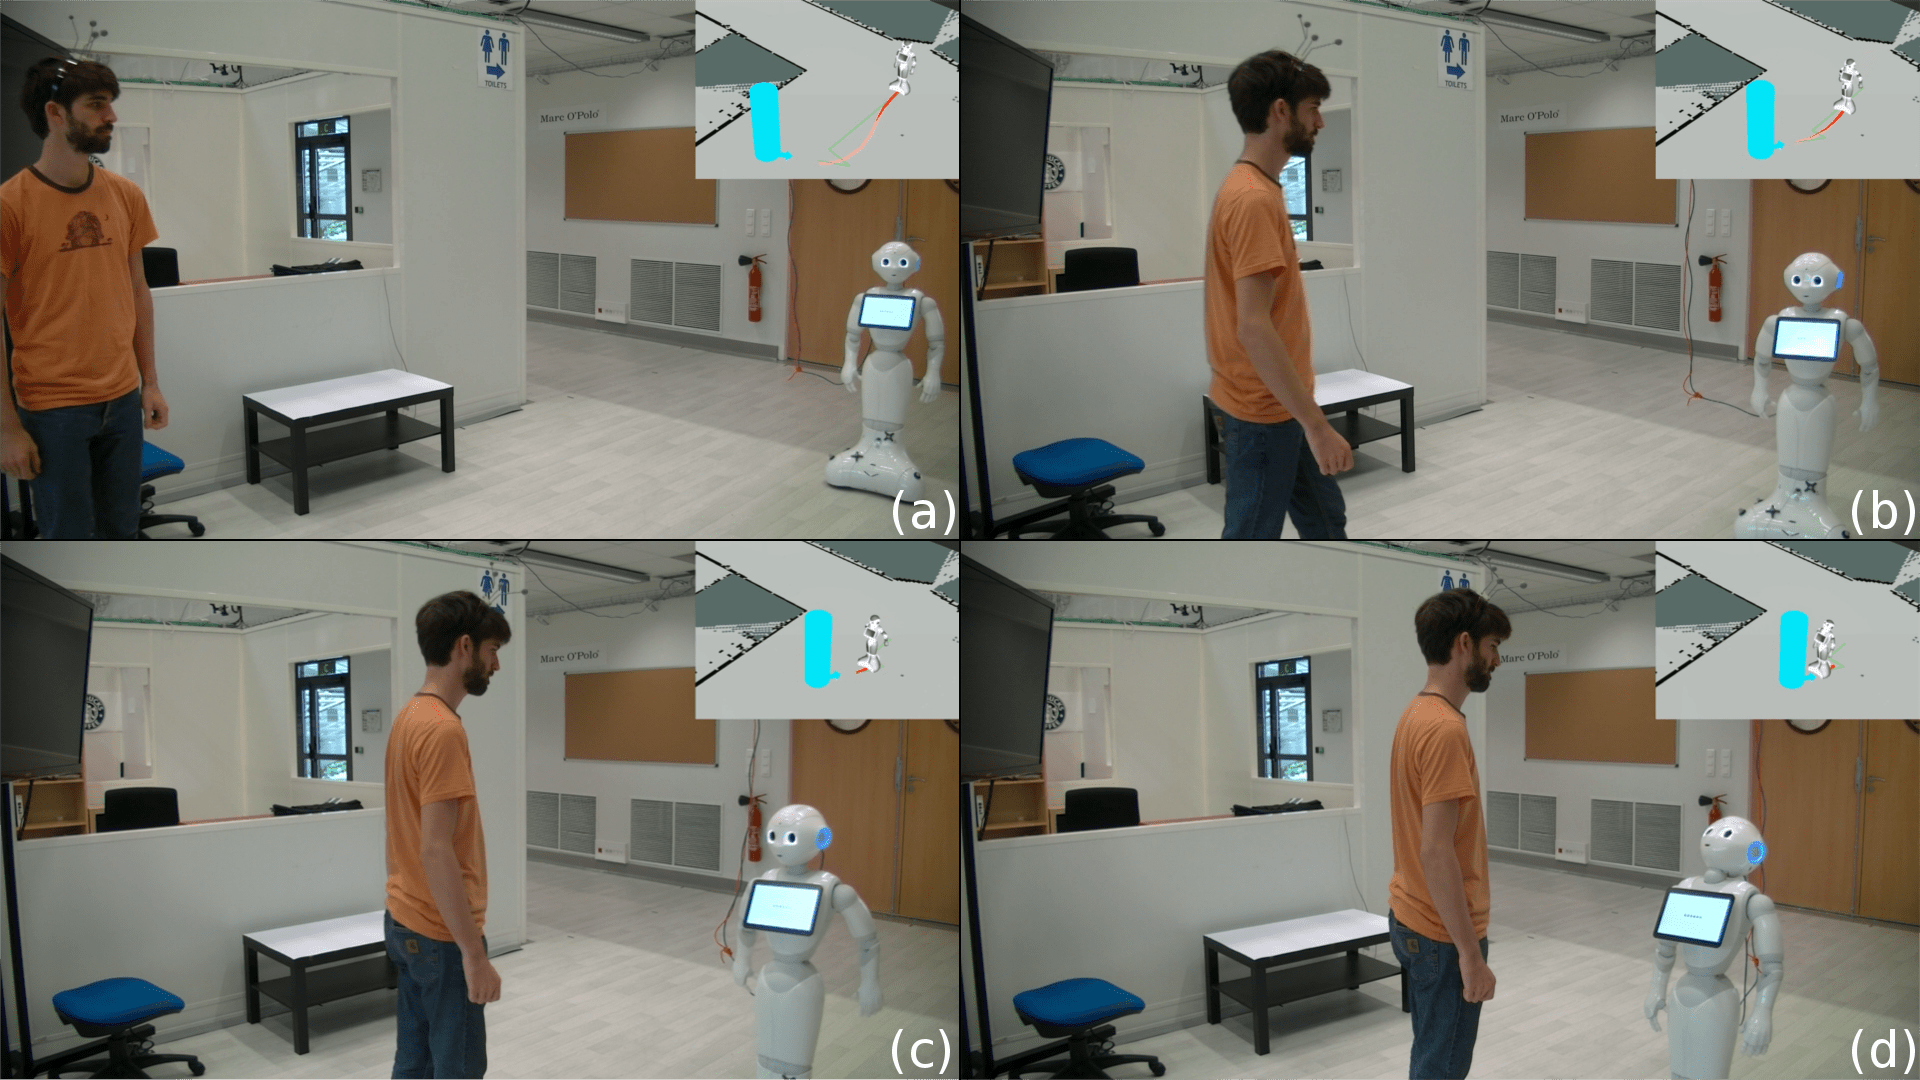
\includegraphics[width=\textwidth]{figures/chapter2/approach.png}
\caption{The Pepper robot approaching a human. The planner adapts to the human moves. In (a) the planned path is long but decrease in (b) and (c) as the human is actively taking part in the approach task until it successfully reaches a position close in front of the human (d).}
\label{fig:approach}
\end{figure}


While this scheme worked well for the approach, with the robot presenting an efficient approach trajectory reacting the human motion (Figure~\ref{fig:approach}), it performed very poorly for the navigation part. Indeed, the robot navigation was erratic and made too long trajectories even between close start and goal points. We identified two causes to this over conservative behavior:

\begin{itemize}
\item First, the \acrshort{hateb} algorithm did not support holonomic motion. Although this was not a problem for long distance scenarios, it made the robot having to maneuver to achieve small displacements.

\item Then, by planning these short trajectories so close to the human, the optimizer does not have a lot of latitude to play with, and the search space is very noisy and chaotic.
\end{itemize}

It has thus been decided in the project to not use \acrshort{hateb}, but simply an holonomic timed elastic band enriched with social constraints linked to the nearby humans (\textit{i.e.} only optimizing the robot trajectory and not the human one).

This allowed to point out some of the limitations of \acrshort{hateb}, it performs poorly for small, intricate displacements. This led to the creation of HATEB2 \cite{singamaneni2020hateb}, which is able to switch online between the \acrshort{hateb} planner, the \acrshort{teb} planner with social constraints or a velocity obstacle planner. Moreover, tracking the human position was really challenging. Indeed, we were provided with a human detection system based on the head mounted camera which presented two drawbacks. First, when the robot was moving, the picture was blurred, preventing any human detection. Then, as the robot and the human were moving to the planned pointing position, the human disappeared from the robot field of view. Because of these tracking problems, any navigation scheme using social constraints (based on human position) revealed hard to use.

\subsection{Using the Estimated Time to Goal to Measure the Execution of the Planned Trajectory}

Another benefit of the \acrshort{hateb} approach is that it does not only compute speed command to follow a global plan while avoiding obstacles like other classic local planner, but also returns a complete short term trajectory for both the robot and the human. Moreover, as the trajectories contains the expected duration between each pose, simply by summing them, we can have an estimate of the time remaining to execute the local trajectories. Besides, we also compute the estimated time remaining for the global trajectories after the local ones by dividing the computed speed at the last local trajectory pose by its length. By summing these two estimated remaining times, we can have a estimation of the remaining navigation time (the time to goals) for all the considered agents.

By monitoring the evolution of these times, we can estimate a quality of the ongoing navigation. Indeed, the local trajectories are computed at at a position control rate and so are the time to goals. Intuitively, if the computed time to goals are decreasing at the same rate as the real time duration (\textit{e.g.} the estimation for the robot goes from 12 seconds to 11 seconds while one second has elapsed) the execution of the trajectories are going according to plan. Instead, if the computed time to goals are decreasing slower than the real time duration, staying equals or even increasing, the execution does not go as smoothly as the plan was.

We formalized it as follows: 
\begin{equation}
s_i(t) = \frac{ttg_i(t) - ttg_i(t - x)}{x}
\end{equation}
with $s_i(t)$ is the time to goal variation for the trajectory $i$ (either the robot or one of the considered human) at time $t$, and $x$ is the time window size parameter, specifying how old are the previous time to goal value we are comparing the current one with.
With this definition we have:
\begin{itemize}
\item $s(t) \approx 1$: the execution goes according to plan,
\item $s(t) > 1$: the execution outperforms the plan,
\item $0 < s(t) < 1$: the execution goes slower than the plan, but progress towards the goal is still being made,
\item and $s(t) < 0$: the goal is getting further.
\end{itemize}

This value can then be fed back to a supervision system which can change the navigation parameters or abort it to make a repair strategy if, combined with other task monitored values, it judges the navigation action is endangering the higher level task.

From preliminary tests, we saw that this measure is a good indicator of the nominal execution of the plan. However it still has to be refined as the measure can be coarse and does not detect the subtle plan changes. Moreover, even if the evaluation is deteriorating, it does not give insight on why. Indeed, the plan change can be caused by multiple factors. It can be from previously unknown obstacles to the robot leading to a plan change (concerns only $\robotmodel$), not necessary representing a collaboration issue. The deterioration can also be from a plan change from the human, making the robot to adapt to it. Finally, we cannot, based only on this measure, determine if the human is not following the computed plan because the model the robot has is not accurate enough ($\humanmodel$) or because the human is really no willing to cooperate. These questions and a similar approach are part of work continued by Amandine Mayima in order to evaluate the quality of interaction during collaborative tasks execution \cite{mayima2020toward}.

\section{Conclusion}

In this chapter, we presented a robot navigation planner \acrshort{hateb}, which not only computes an optimal local trajectory for the robot but also for the surrounding humans. This approach has been shown to be able to solve complex navigation tasks where both agents must cooperate to reach their respective goals. Moreover, we proved via a user study that it allows to implement effective coordination smoothers to increase the robot mutual manifestness and facilitate the whole interaction.
Besides, the versatility of this approach has been presented via its implementation on three different robots: PR2, HRP2 and Pepper.
Finally, we used an other benefit of this scheme which is to compute precise local trajectory at position control loop rate to estimate the remaining time to reach the navigation goal. By processing this data and monitoring it over the course of interaction, quality of the ongoing navigation and interaction can be deduced and returned to a higher level supervision component. A more general approach including some principles presented here is developed by Amandine Mayima to measure the quality of interaction by a supervision system in real-time during a collaborative task execution~\cite{mayima2020toward}.

The presented navigation approach that plans for both the human and the robot presents some drawbacks. First, through the \acrshort{mummer} project, we saw that it fails to generate small paths when the human and the robot are close to each other. Indeed, such intricate trajectories are complex to optimize as they are heavily constrained. Then, the scheme breaks if the human model parameters are not accurate enough. Indeed, the optimization scheme will assume the human to follow a trajectory respecting these parameters. We plan to update these parameters on a per-human basis during the execution to get the most accurate plan for the human. Finally, the conavigation solutions found are executed as if the human is aware of them. While it allows to check that a solution can exists it does not guarantee that it is the solution the human will choose. In most cases, if the human choose another trajectory than the one planned, the optimizer will adapt, but in some intricate cases, not accounting for the communication needed to share the plan can lead to deadlocks. For navigation, the communication can be explicit by looking at the trajectory chosen by the robot or pointing at the human planned one, but it can also be implicit through the use of coordination smoothers.

We are particularly interested in these coordination smoothers, which can be seen as non verbal communication of the robot intents and of the shared plan. Planning for these coordination smoothers can only be done if we plan for both the robot and the human. However, due to the continuous and short duration nature inherent to navigation tasks, exploring the planning of such communication can be tedious. We thus propose to move from navigation problems to focus on human robot symbolic task planning.


\ifdefined\included
\else
\bibliographystyle{acm}
\bibliography{These}
\end{document}
\fi
